\section{Results and Evaluation}

\subsection{Demand and Response-Performance Patterns}

The canonical slice contains 293{,}646 incidents across 33 London local-authority areas from January 2024 to 27 February 2026; the last month is partial. Among 278{,}468 rows with a recorded first-pump time, the author's incident-level share above 360 seconds is 32.4\% (95\% Wilson CI 32.3--32.6\%). This is a diagnostic based on the numerical value of LFB's pan-London average target, not an official per-incident failure rate. False alarms form 46.5\% of incidents, so the dashboard retains incident group in every comparison.

\begin{figure}[H]
\centering
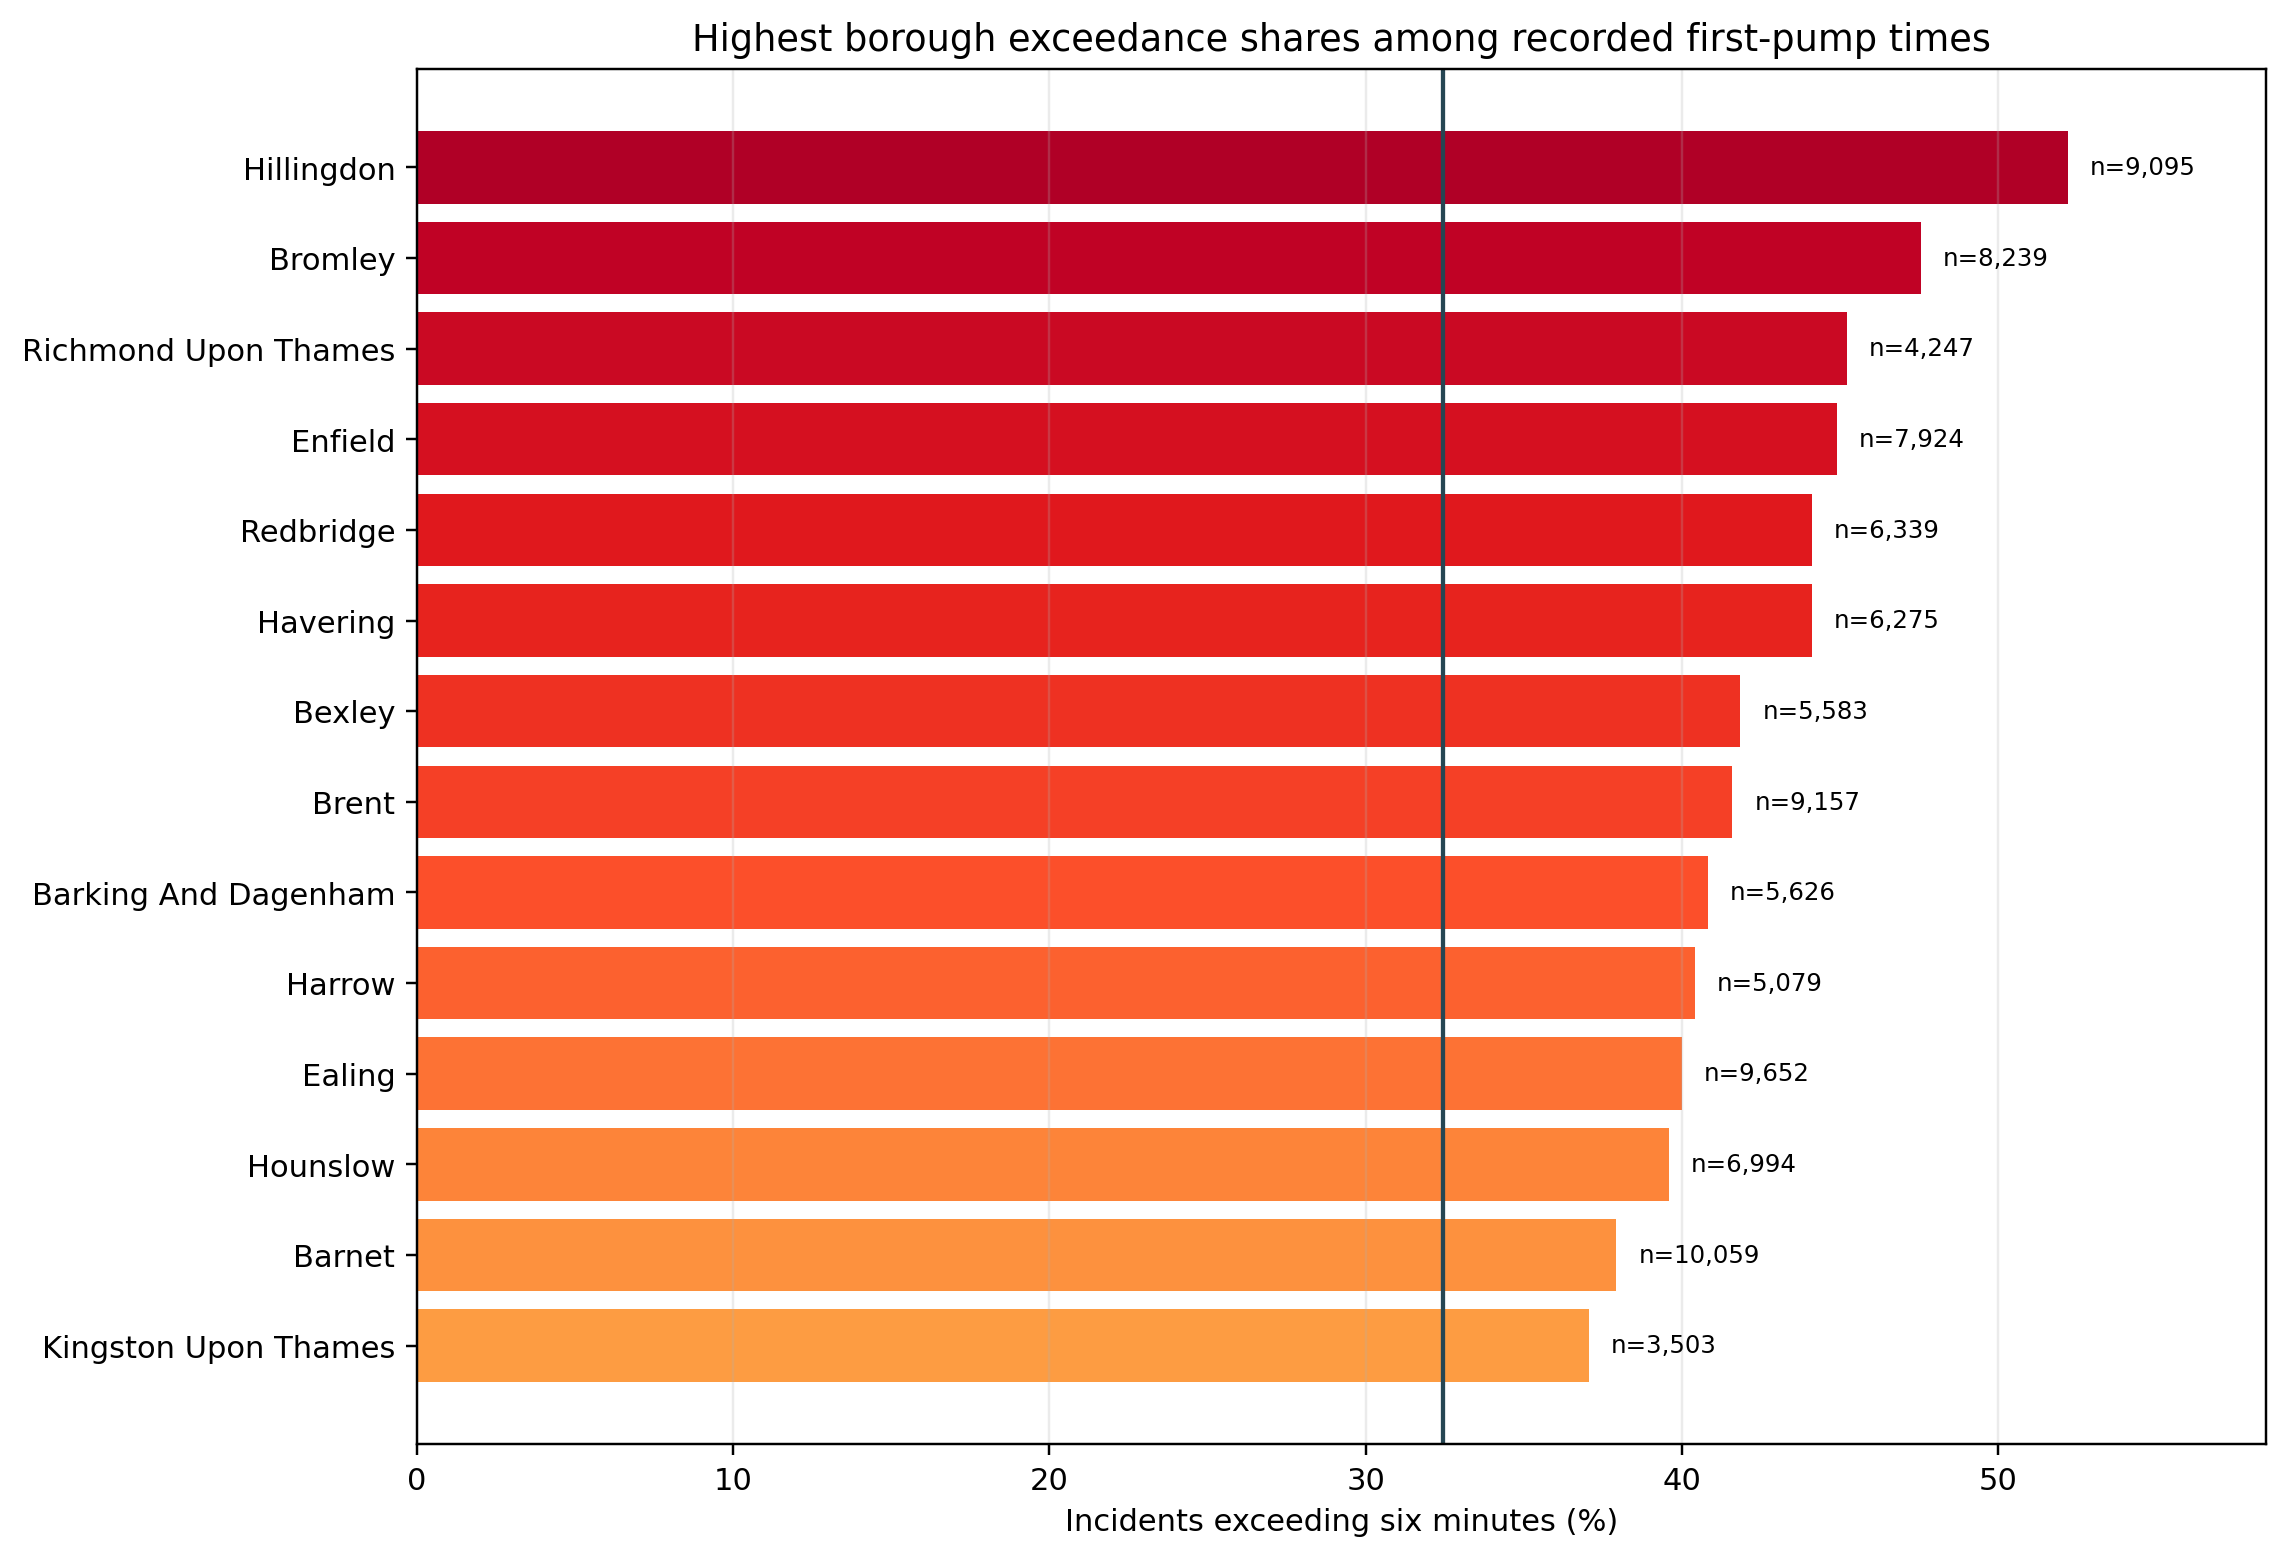
\includegraphics[width=\textwidth]{figures/results_evaluation/fig_borough_exceedance_ranking.png}
\caption{Highest borough values of the author-derived incident diagnostic. Bars show the share above 360 seconds among recorded first-pump times; whiskers are 95\% Wilson intervals and labels give recorded $n$.}
\label{fig:borough-exceedance-ranking}
\end{figure}

Figure~\ref{fig:borough-exceedance-ranking} turns the ranking into a static result. Hillingdon is highest at 52.2\% ($n=9{,}095$, 95\% CI 51.2--53.2\%), followed by Bromley at 47.6\% and Richmond upon Thames at 45.2\%. Kensington and Chelsea is lowest at 17.9\%. These are borough-level response-performance disparities; an equity interpretation would require additional measures of population need and distribution.

\begin{figure}[H]
\centering
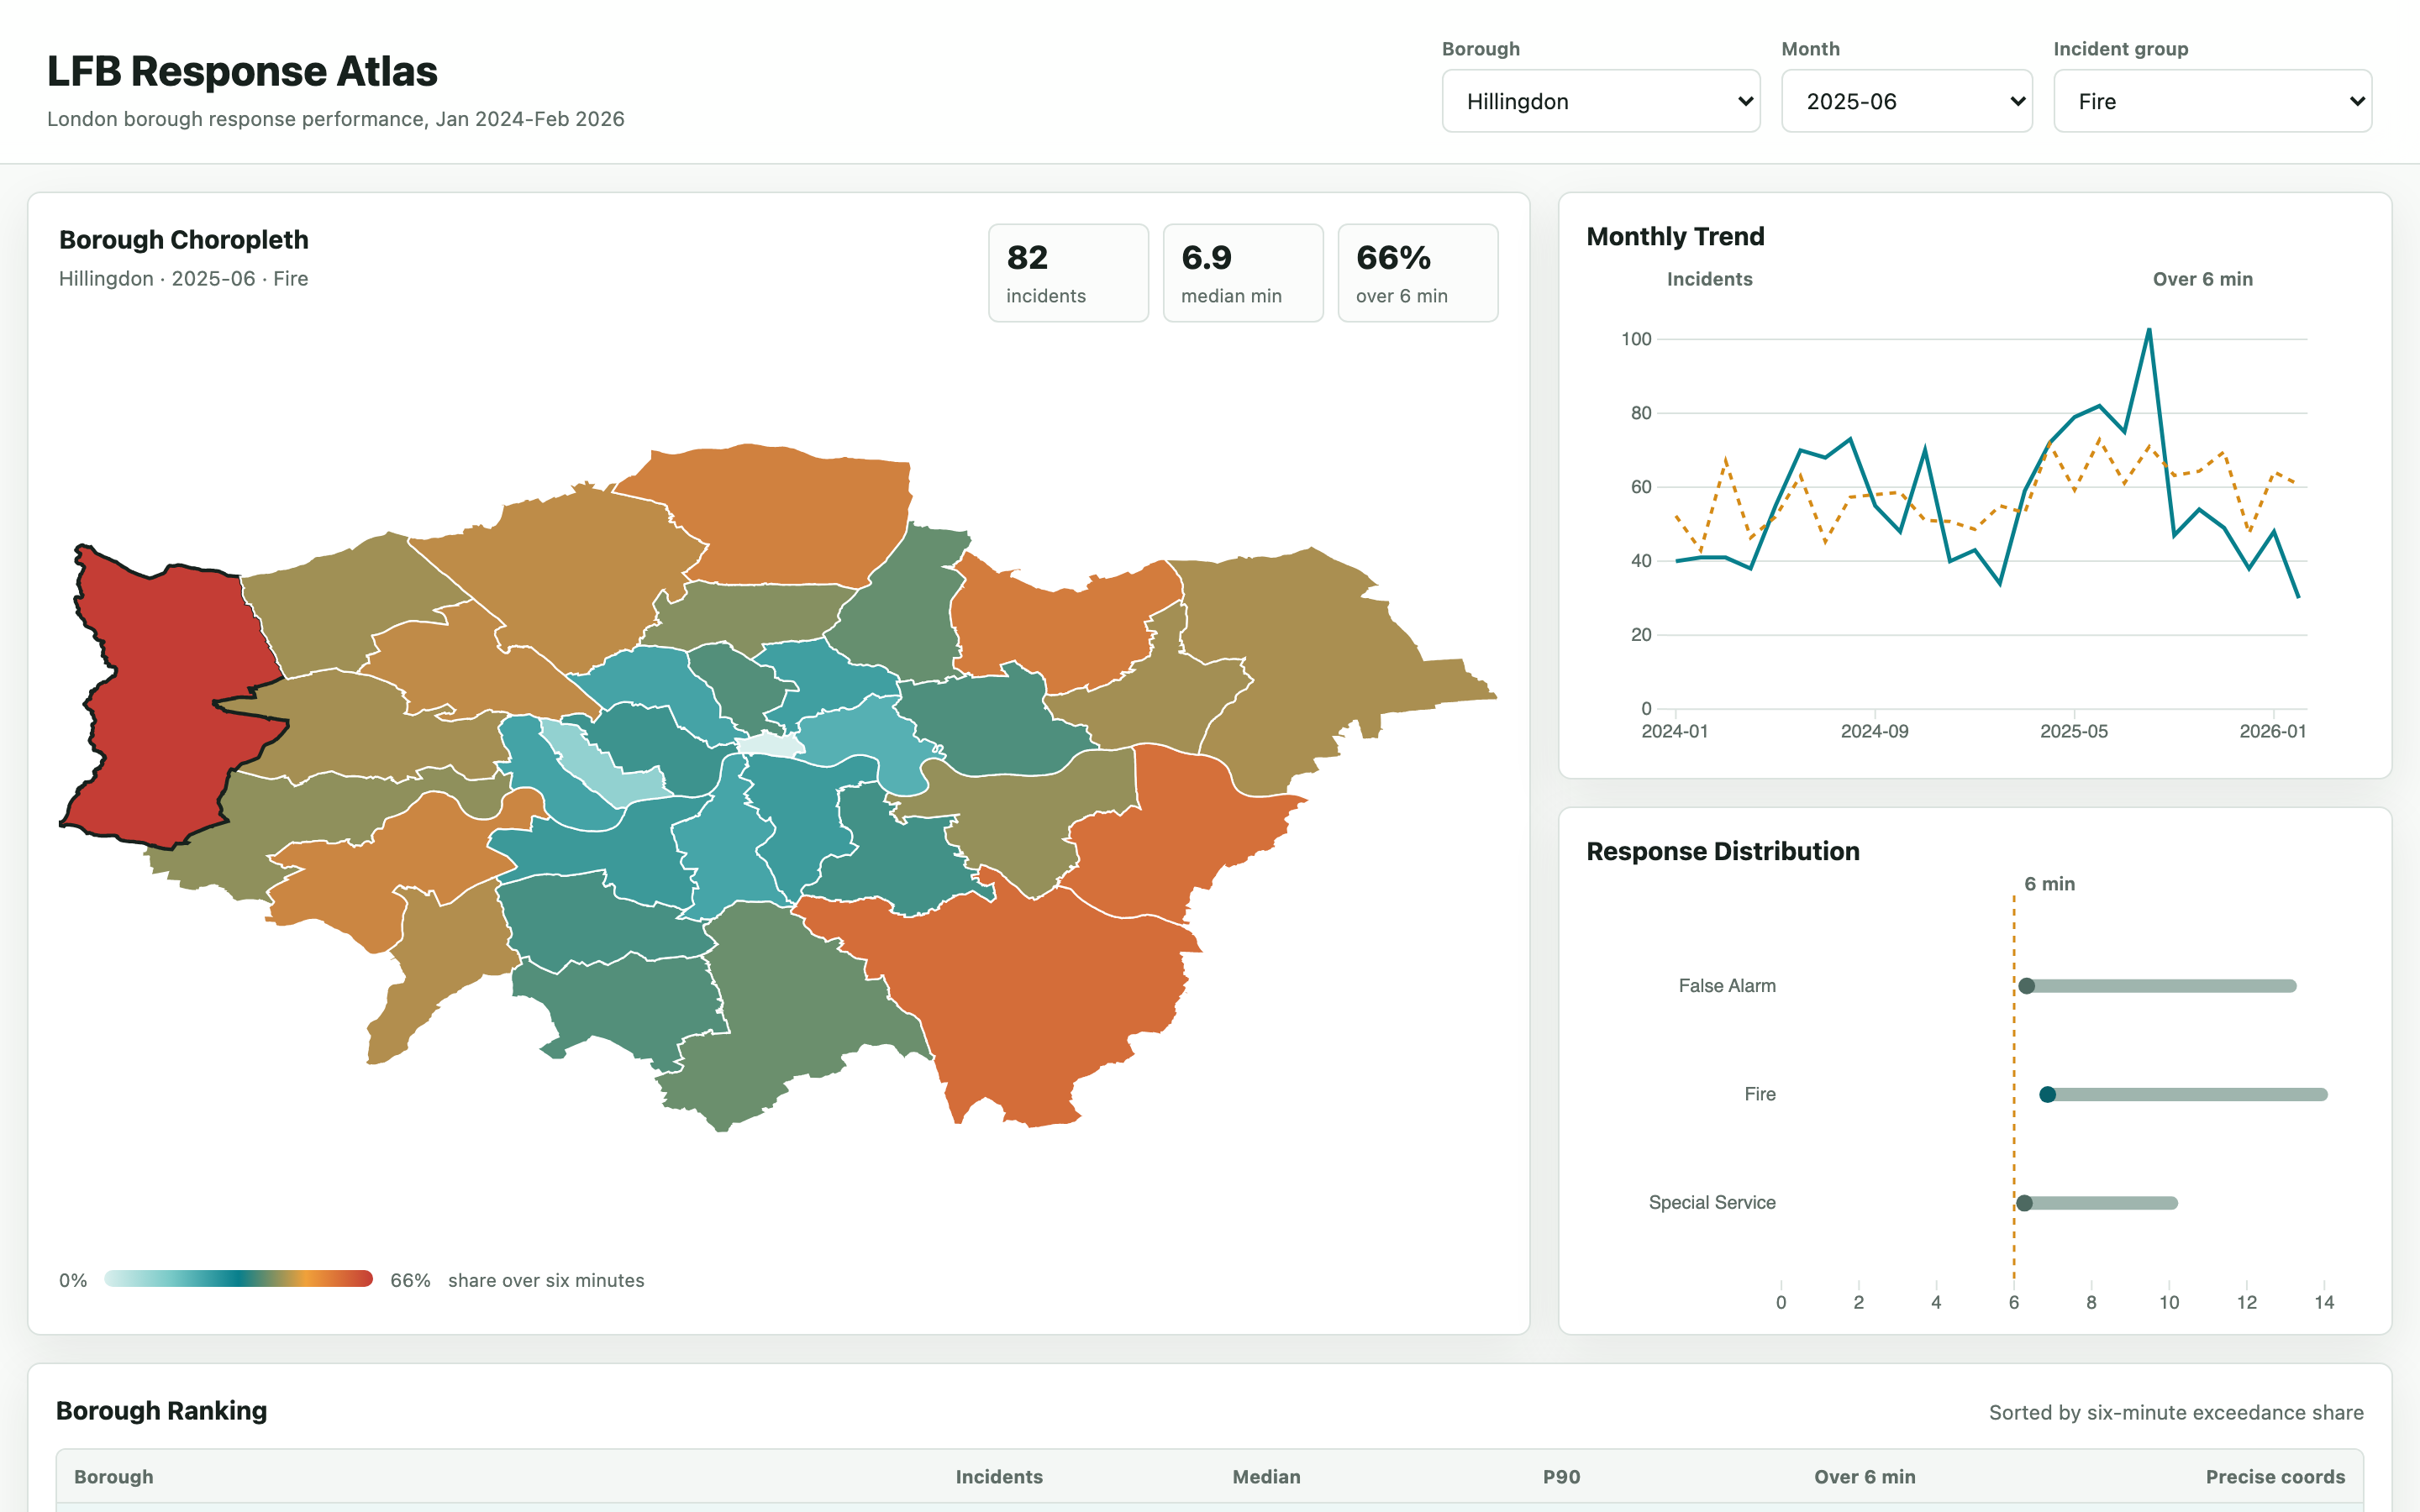
\includegraphics[width=\textwidth]{figures/dashboard/fig_dashboard_overview_desktop.png}
\caption{Dashboard overview of the linked borough map, trend, distribution, and ranking panels. Response summaries use recorded first-pump times; February 2026 is marked as partial.}
\label{fig:dashboard-overview}
\end{figure}

The dashboard treats borough, month, and incident group as the interactive unit. The map shows the spatial contrast, the trend keeps time in view, the distribution shows median-to-p95 spread against a six-minute reference, and the table supplies exact estimates and intervals.

\begin{figure}[H]
\centering
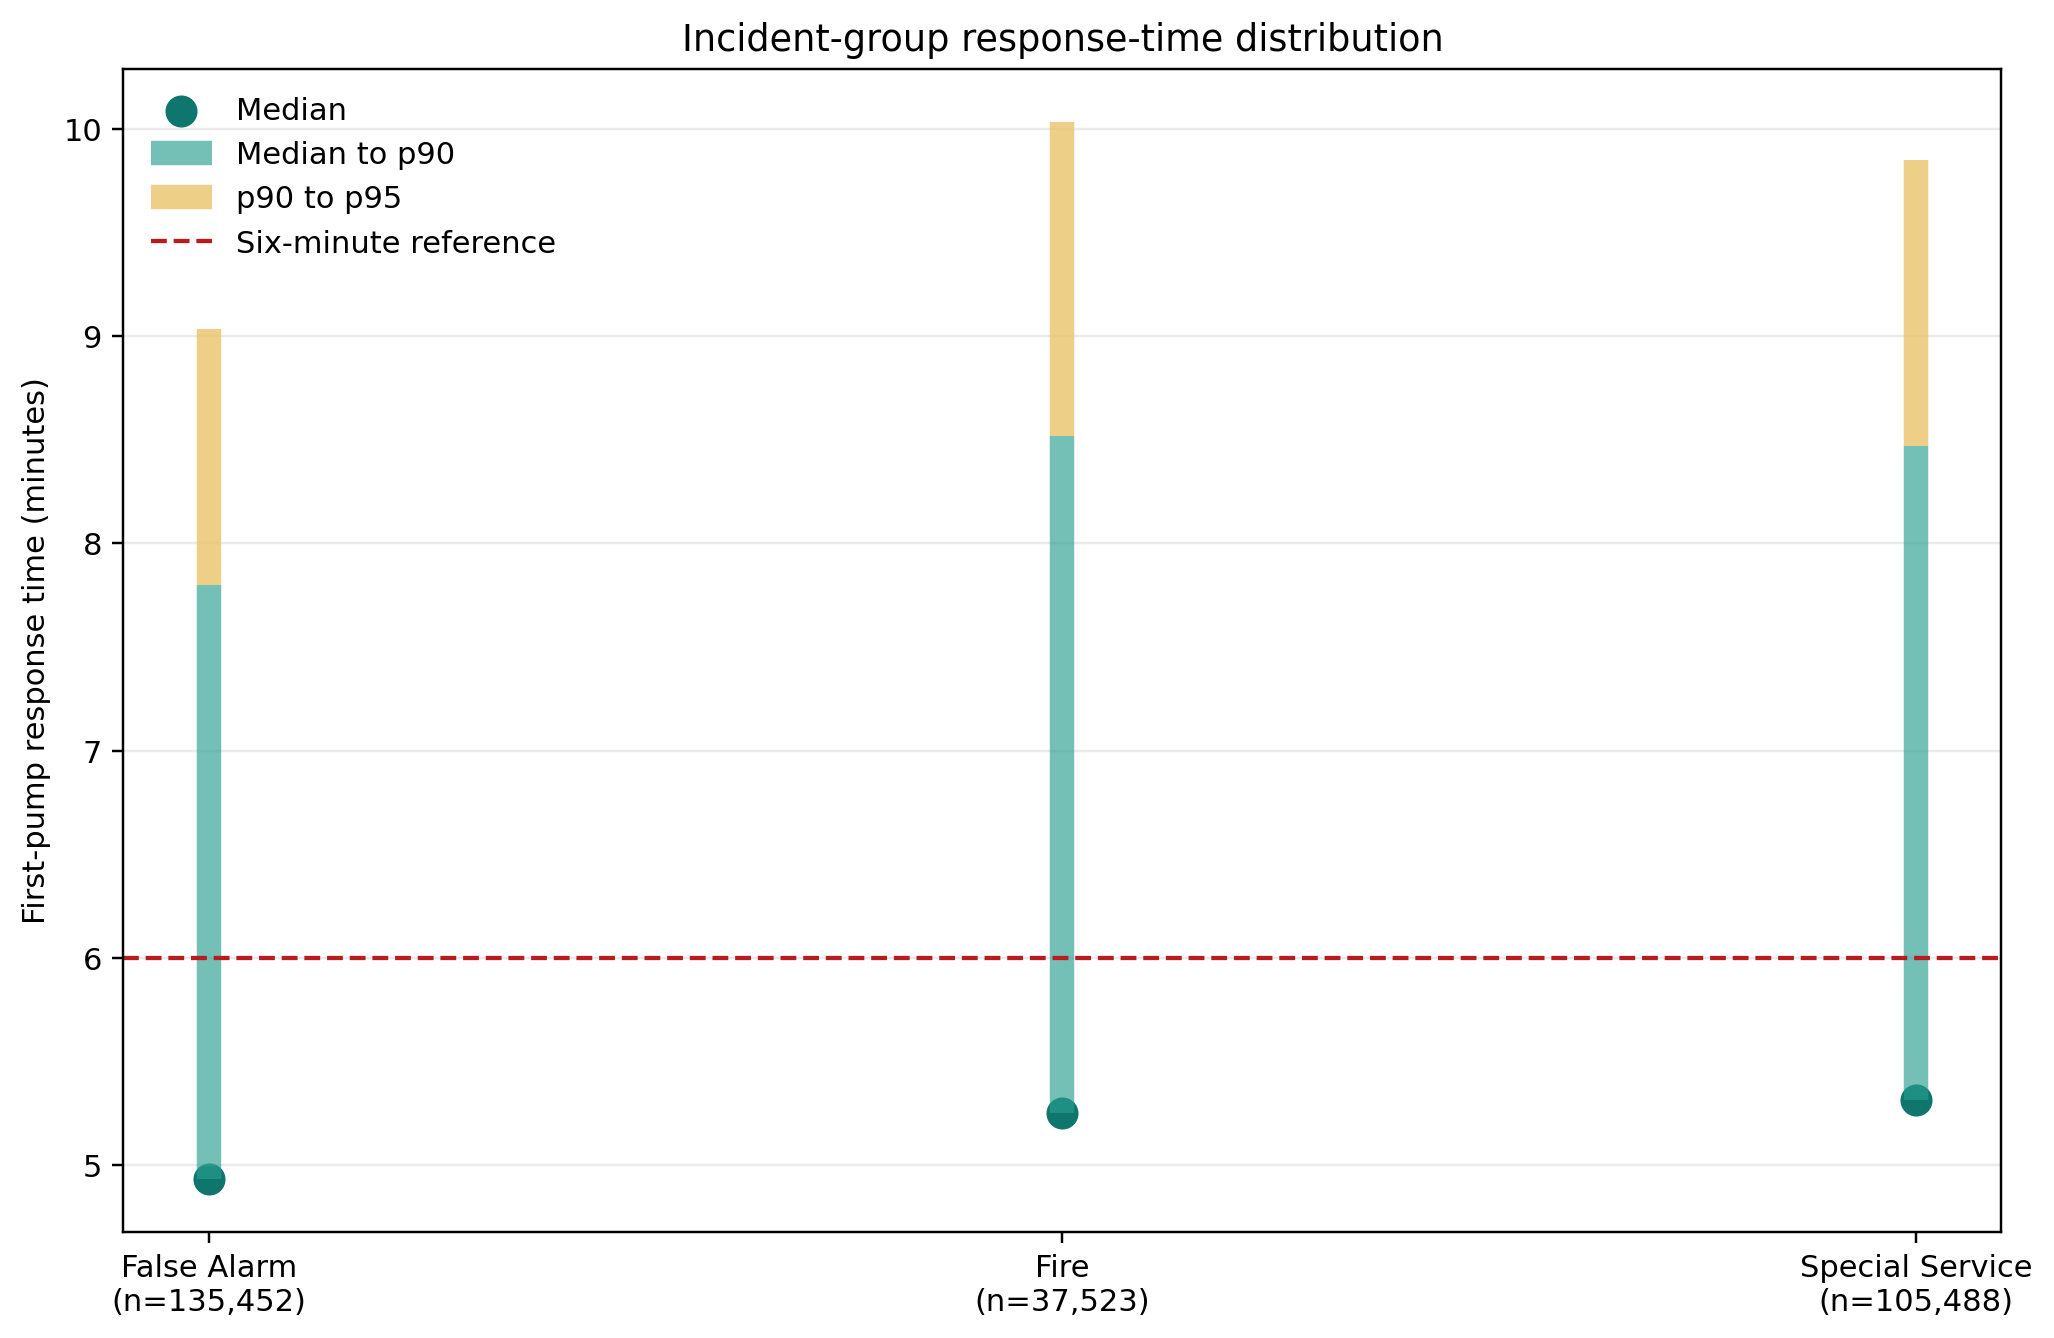
\includegraphics[width=0.88\textwidth]{figures/results_evaluation/fig_incident_group_response_distribution.png}
\caption{Incident-group response-time distribution among incidents with recorded first-pump attendance time. Markers show medians, vertical ranges show median--p90 and p90--p95, and the dashed line uses six minutes as a descriptive reference.}
\label{fig:incident-group-response-distribution}
\end{figure}

The incident-group distribution in Figure~\ref{fig:incident-group-response-distribution} explains why the dashboard keeps incident type in view. Median first-pump response times sit below six minutes for all three groups, but the p90 and p95 values sit above that reference, so a median-only interface would hide the tail that drives exceedance concerns. Fire incidents have a slightly higher median and tail than false alarms, but all three groups require the same denominator discipline: the plotted statistics use recorded first-pump times only.

\begin{figure}[H]
\centering
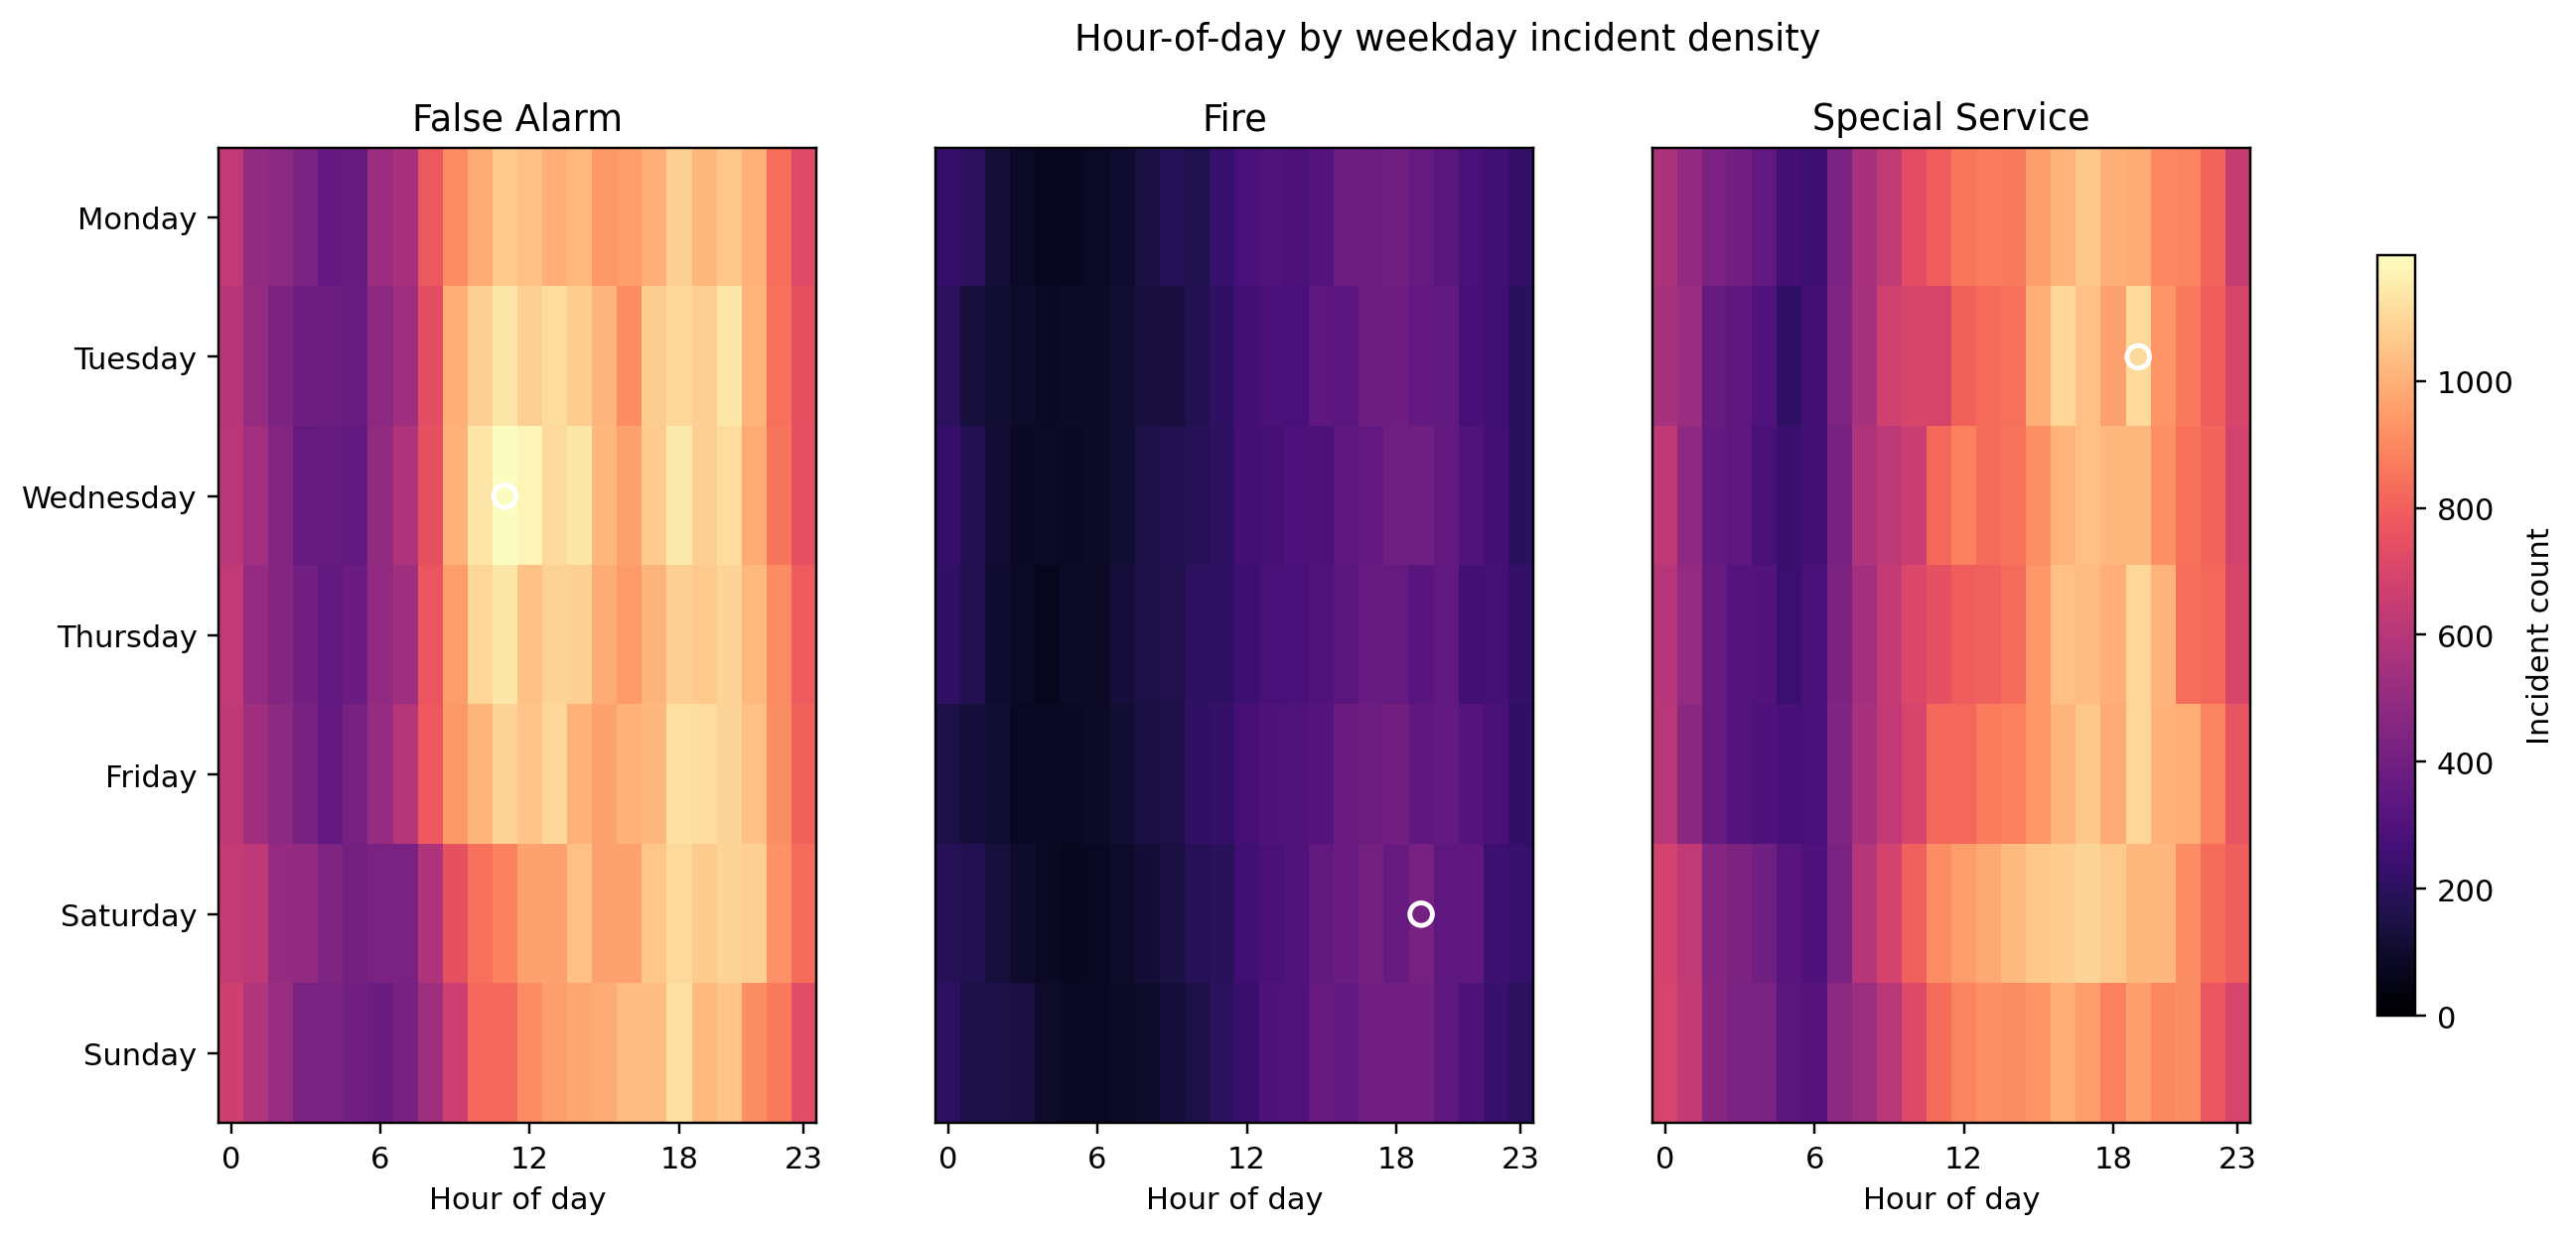
\includegraphics[width=\textwidth]{figures/results_evaluation/fig_temporal_incident_density_heatmap.png}
\caption{Hour-of-day by weekday incident-density heatmaps by incident group. The white ring marks the highest-count cell in each incident-group panel.}
\label{fig:temporal-density-heatmap}
\end{figure}

False alarms peak on Wednesday at 11:00, fire incidents on Saturday at 19:00, and special-service incidents on Tuesday at 19:00 (Figure~\ref{fig:temporal-density-heatmap}). False-alarm demand is strongest in daytime institutional hours, while fires and special services show more evening concentration.

\begin{figure}[H]
\centering
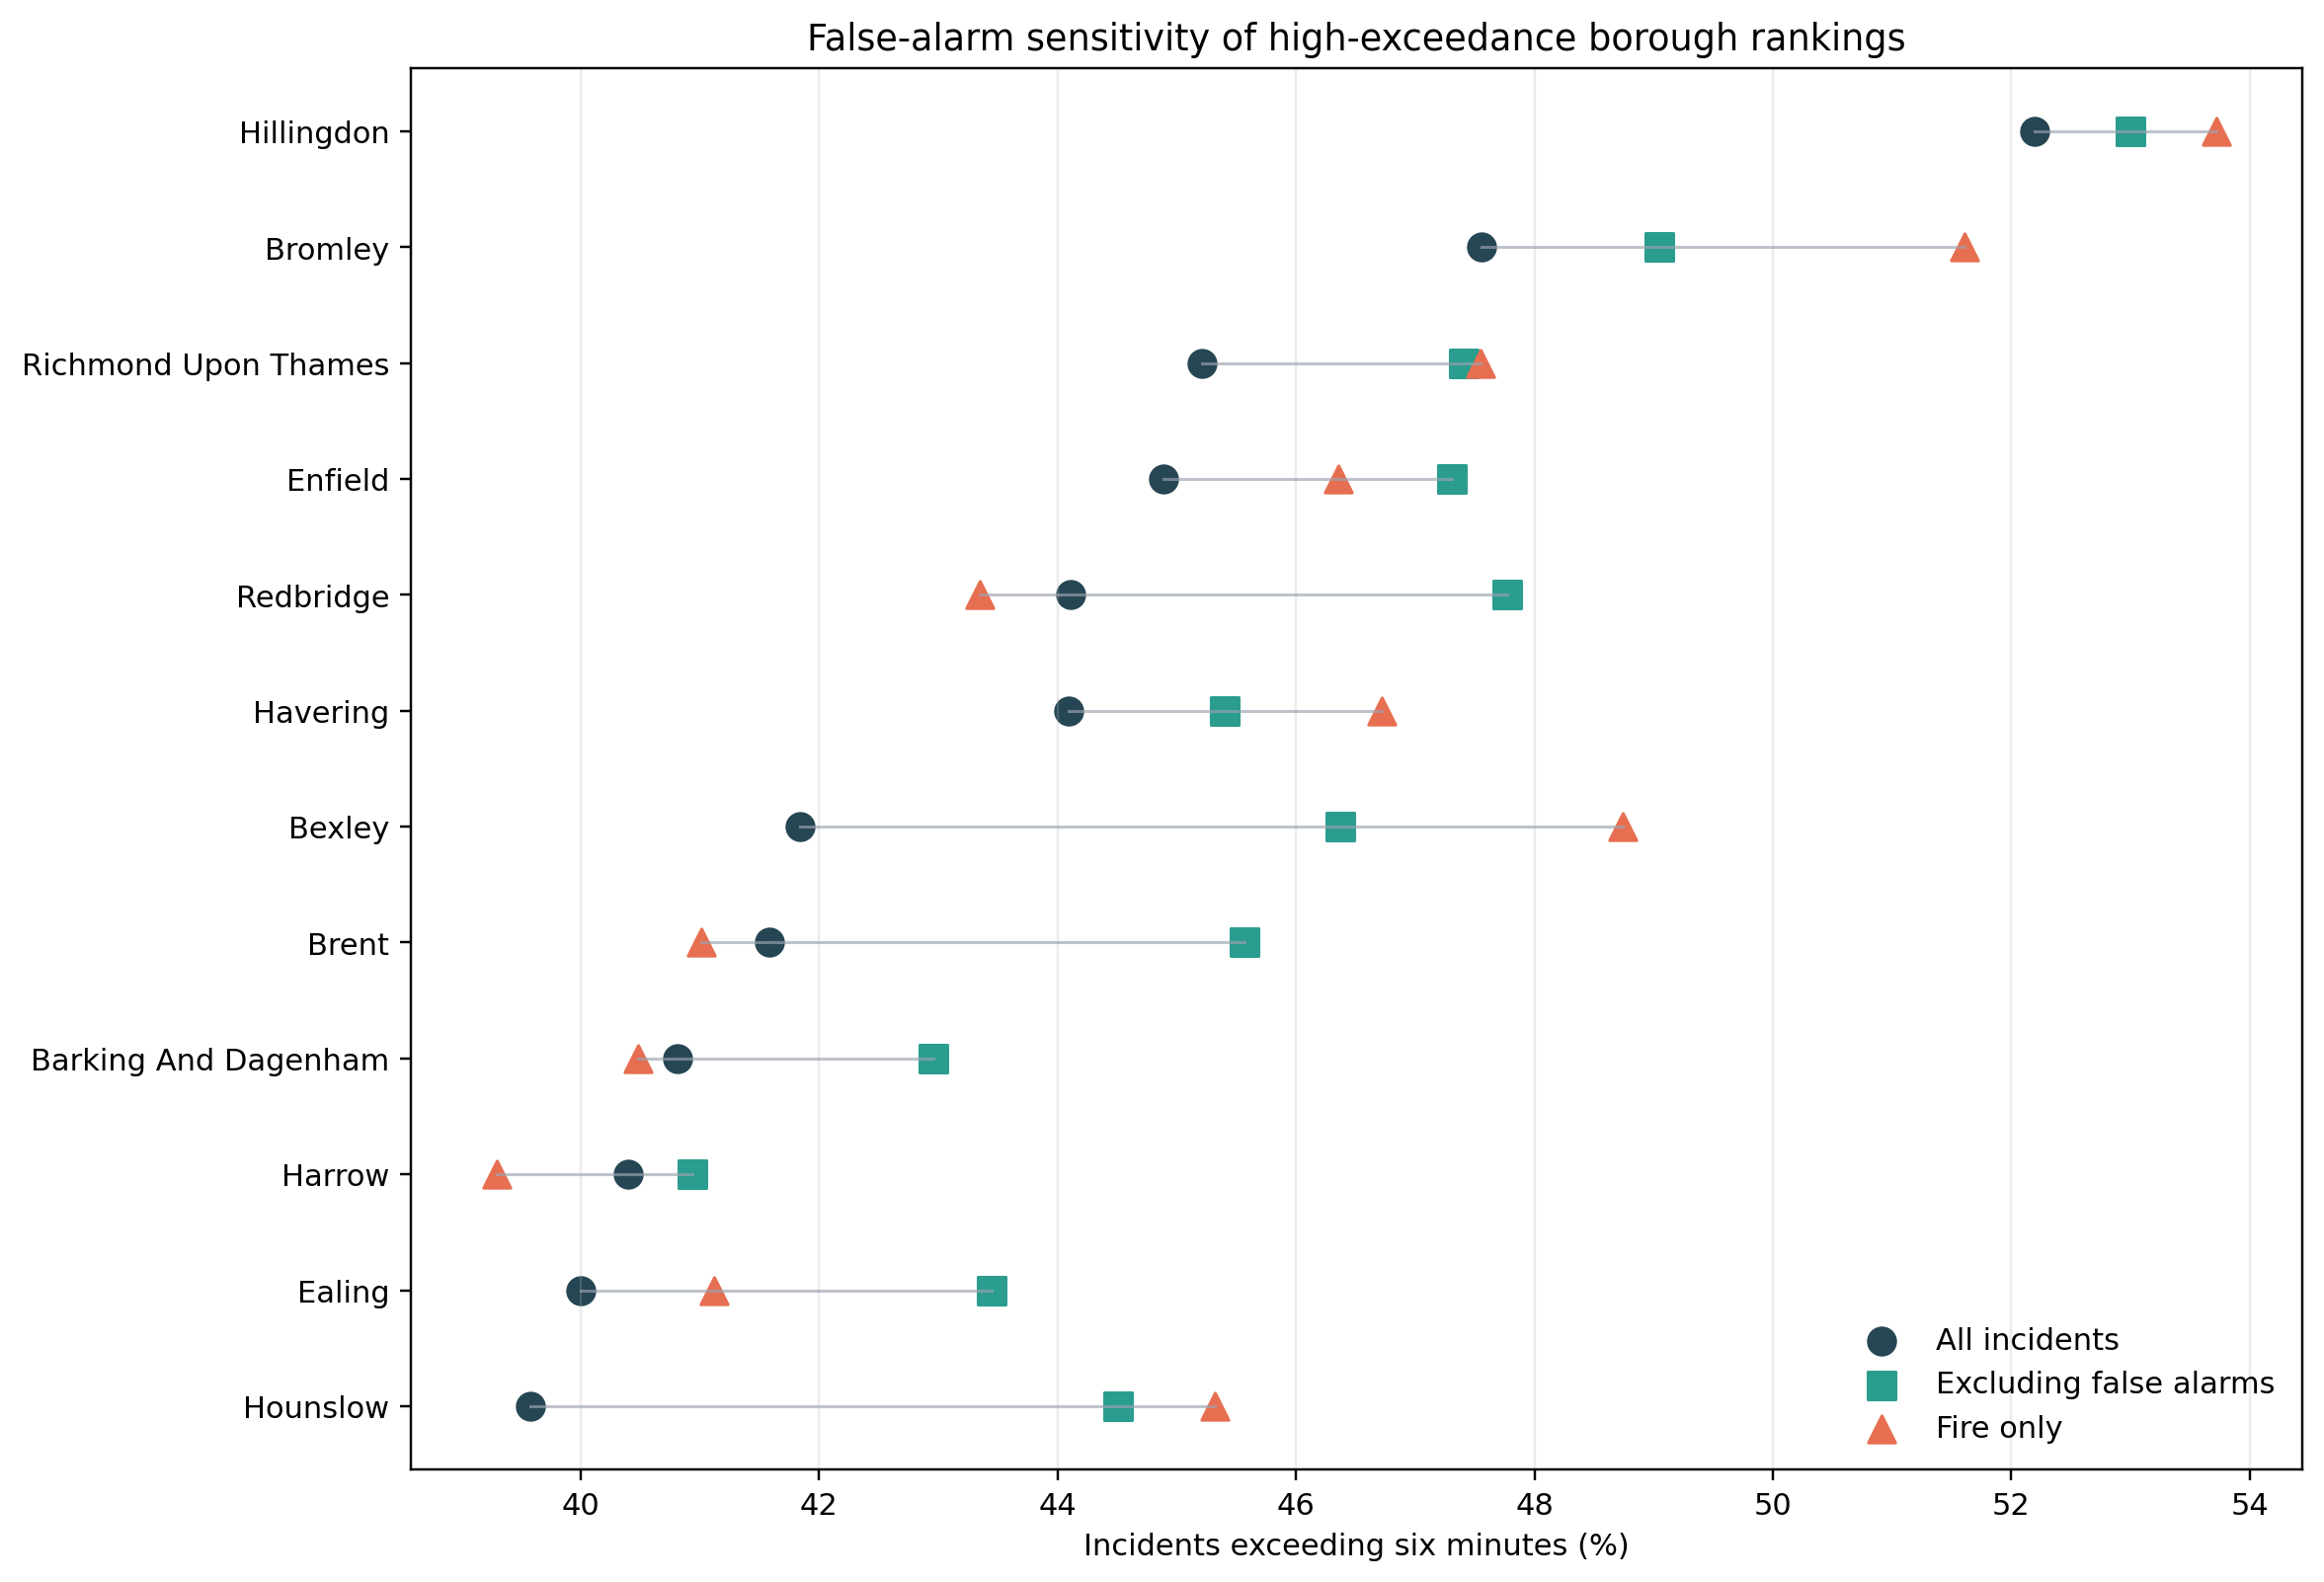
\includegraphics[width=\textwidth]{figures/results_evaluation/fig_false_alarm_sensitivity_ranking.png}
\caption{Sensitivity of high-exceedance boroughs to the false-alarm denominator. Each row compares all incidents, all non-false-alarm incidents, and fire-only incidents for the same borough.}
\label{fig:false-alarm-sensitivity}
\end{figure}

The false-alarm sensitivity check in Figure~\ref{fig:false-alarm-sensitivity} tests whether the headline ranking is driven by false alarms. The ranking is stable at the borough level: Spearman rank correlation is 0.991 between the all-incident and excluding-false-alarm rankings, and 0.970 between the all-incident and fire-only rankings. The largest rank movement when false alarms are excluded is three places. False alarms remain a substantial part of workload, but they do not create the outer-borough pattern on their own.

\begin{figure}[H]
\centering
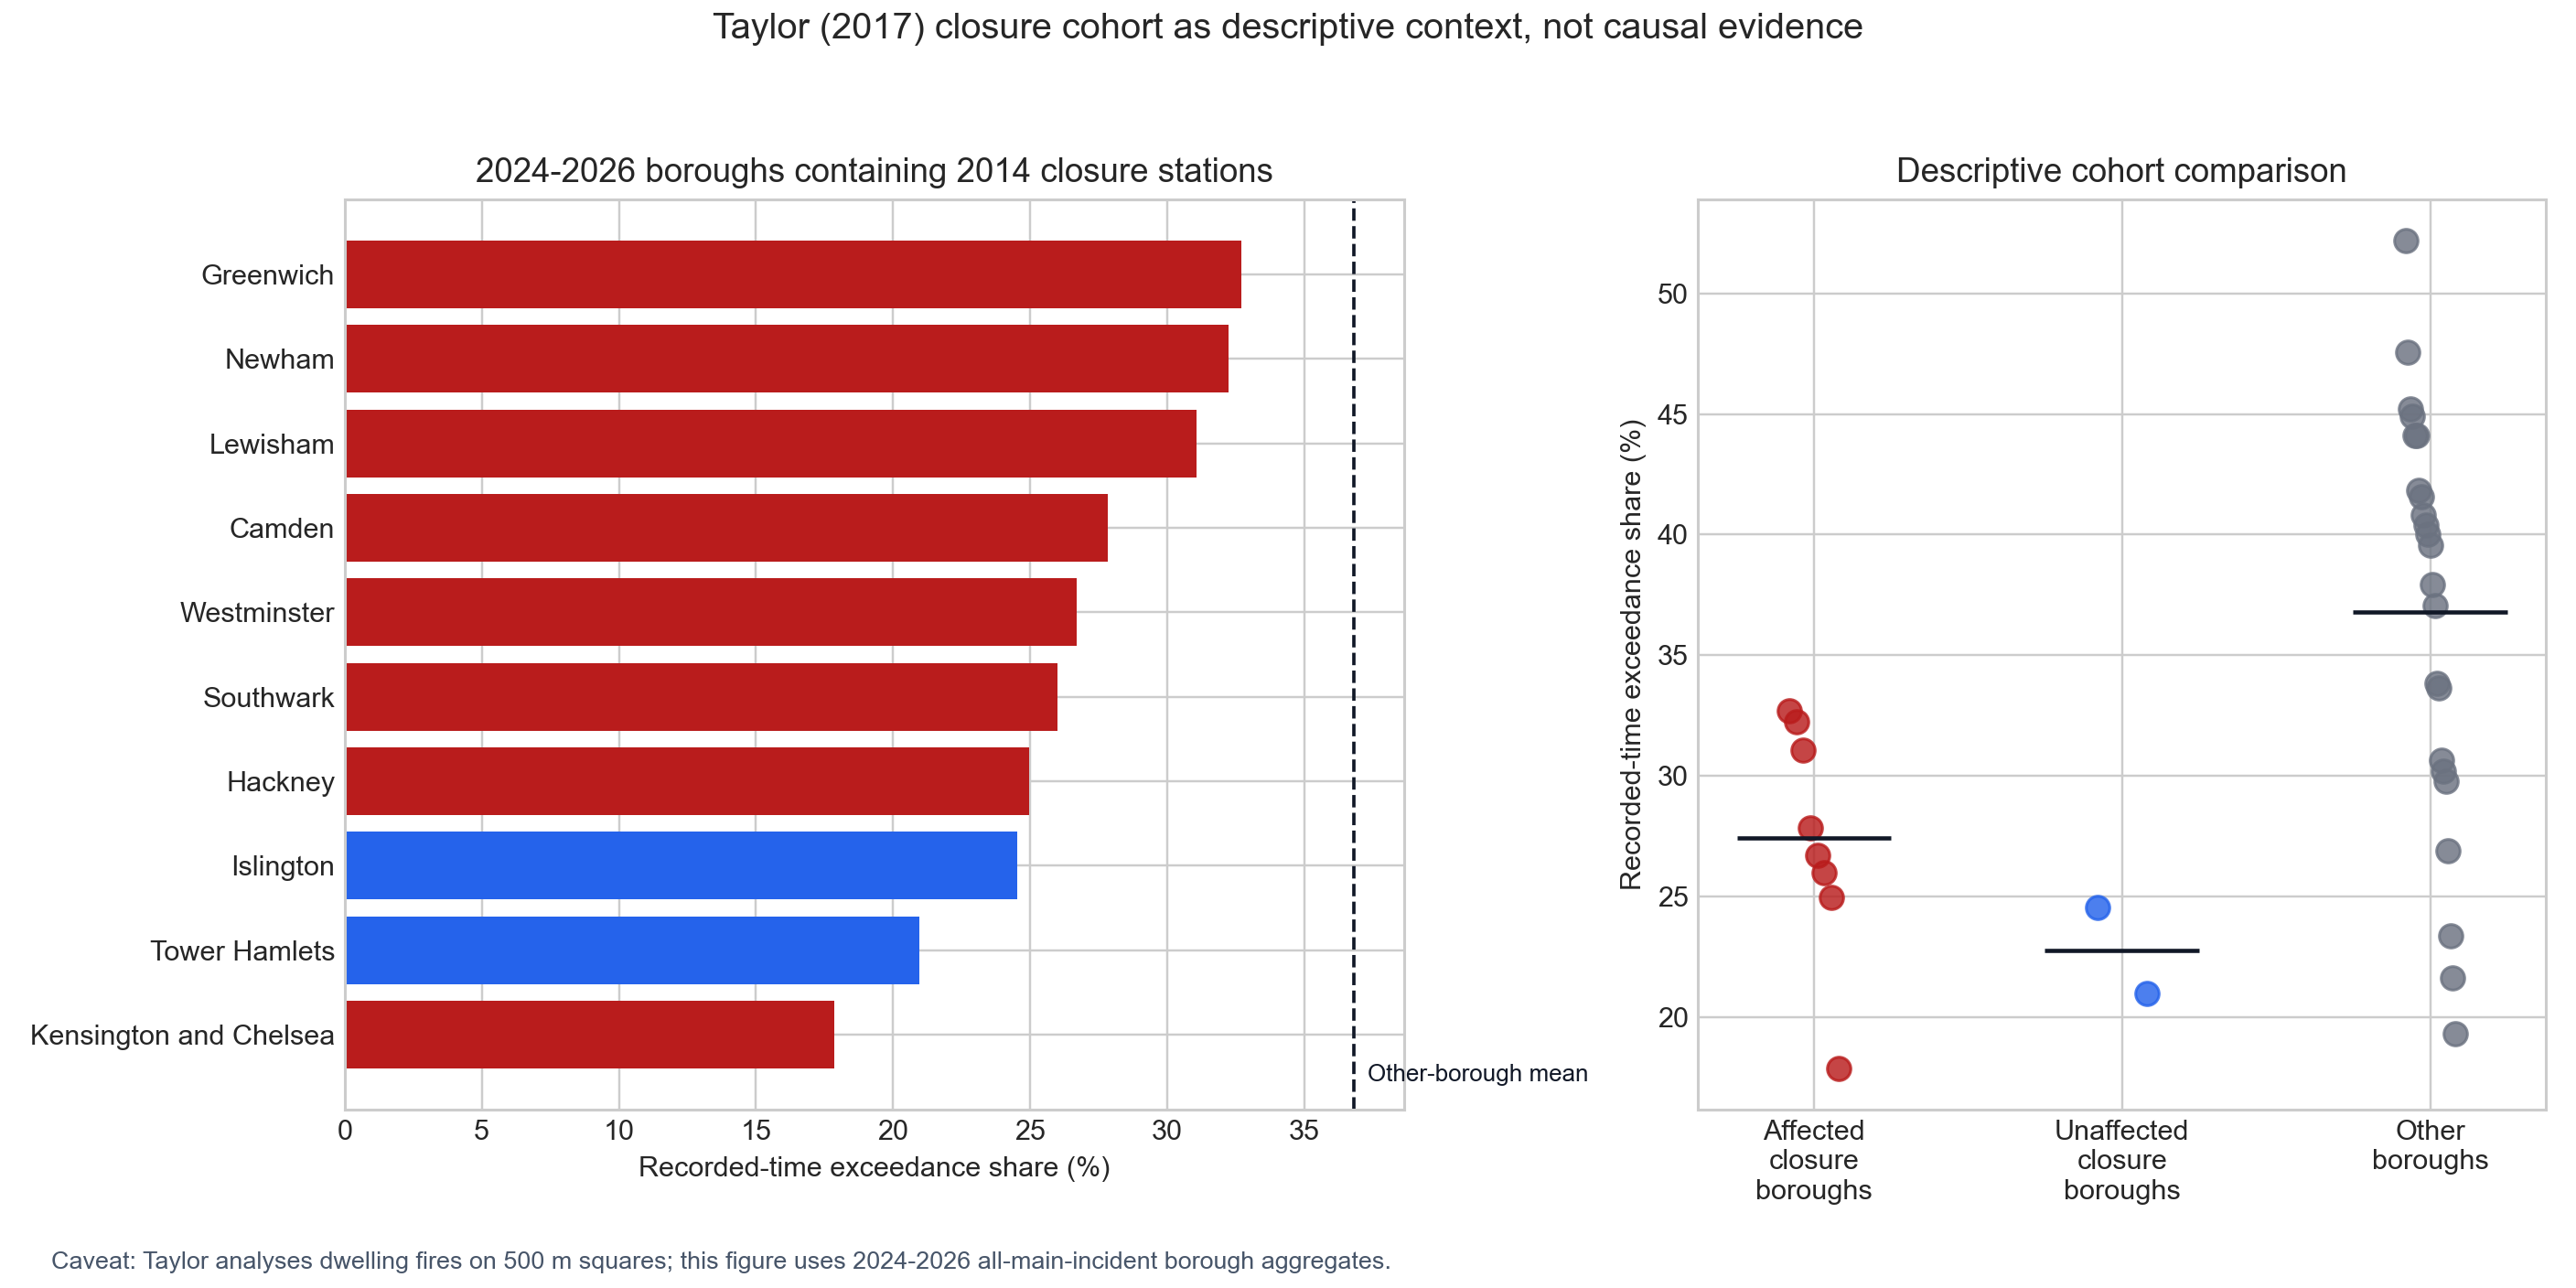
\includegraphics[width=\textwidth]{figures/results_evaluation/fig_taylor_closure_cohort_context.png}
\caption{Descriptive cross-check against Taylor's 2014 closure cohort~\cite{spatial2015}. Boroughs containing Taylor-affected and Taylor-unaffected closed stations are compared with other boroughs using 2024--2026 recorded-time exceedance shares.}
\label{fig:taylor-closure-cohort-context}
\end{figure}

Figure~\ref{fig:taylor-closure-cohort-context} provides a historical cross-check. Boroughs containing Taylor-affected closure stations have a mean recorded-time exceedance share of 27.4\% in the present slice, below the other-borough mean of 36.8\%; the two boroughs containing Taylor-unaffected closure stations average 22.8\%. Taylor models dwelling fires on 500\,m grid squares in 2012--2014, whereas this comparison uses all main incident groups at borough level in 2024--2026. The current averages therefore cannot explain the effect estimated by Taylor. The affected/unaffected labels were checked against the 2017 paper, and the station-to-borough mapping against the official closure listing retained in the provenance sidecar.

The mobilisation table adds appliance-level deployment and arrival fields to the incident summary. Of its rows, 438{,}211 match canonical incidents; 1{,}763 cross-boundary or unmatched rows are retained separately. Deployment summaries in this report use the \path{matches_canonical_incident == True} partition.

\subsection{Station-Address Proximity and the D1 Recovery}

The station-address check (\S5.6) compares incident-derived footprints with postcode centroids from the historical June 2017 file. It supplies a second historical reference point.

\begin{figure}[H]
\centering
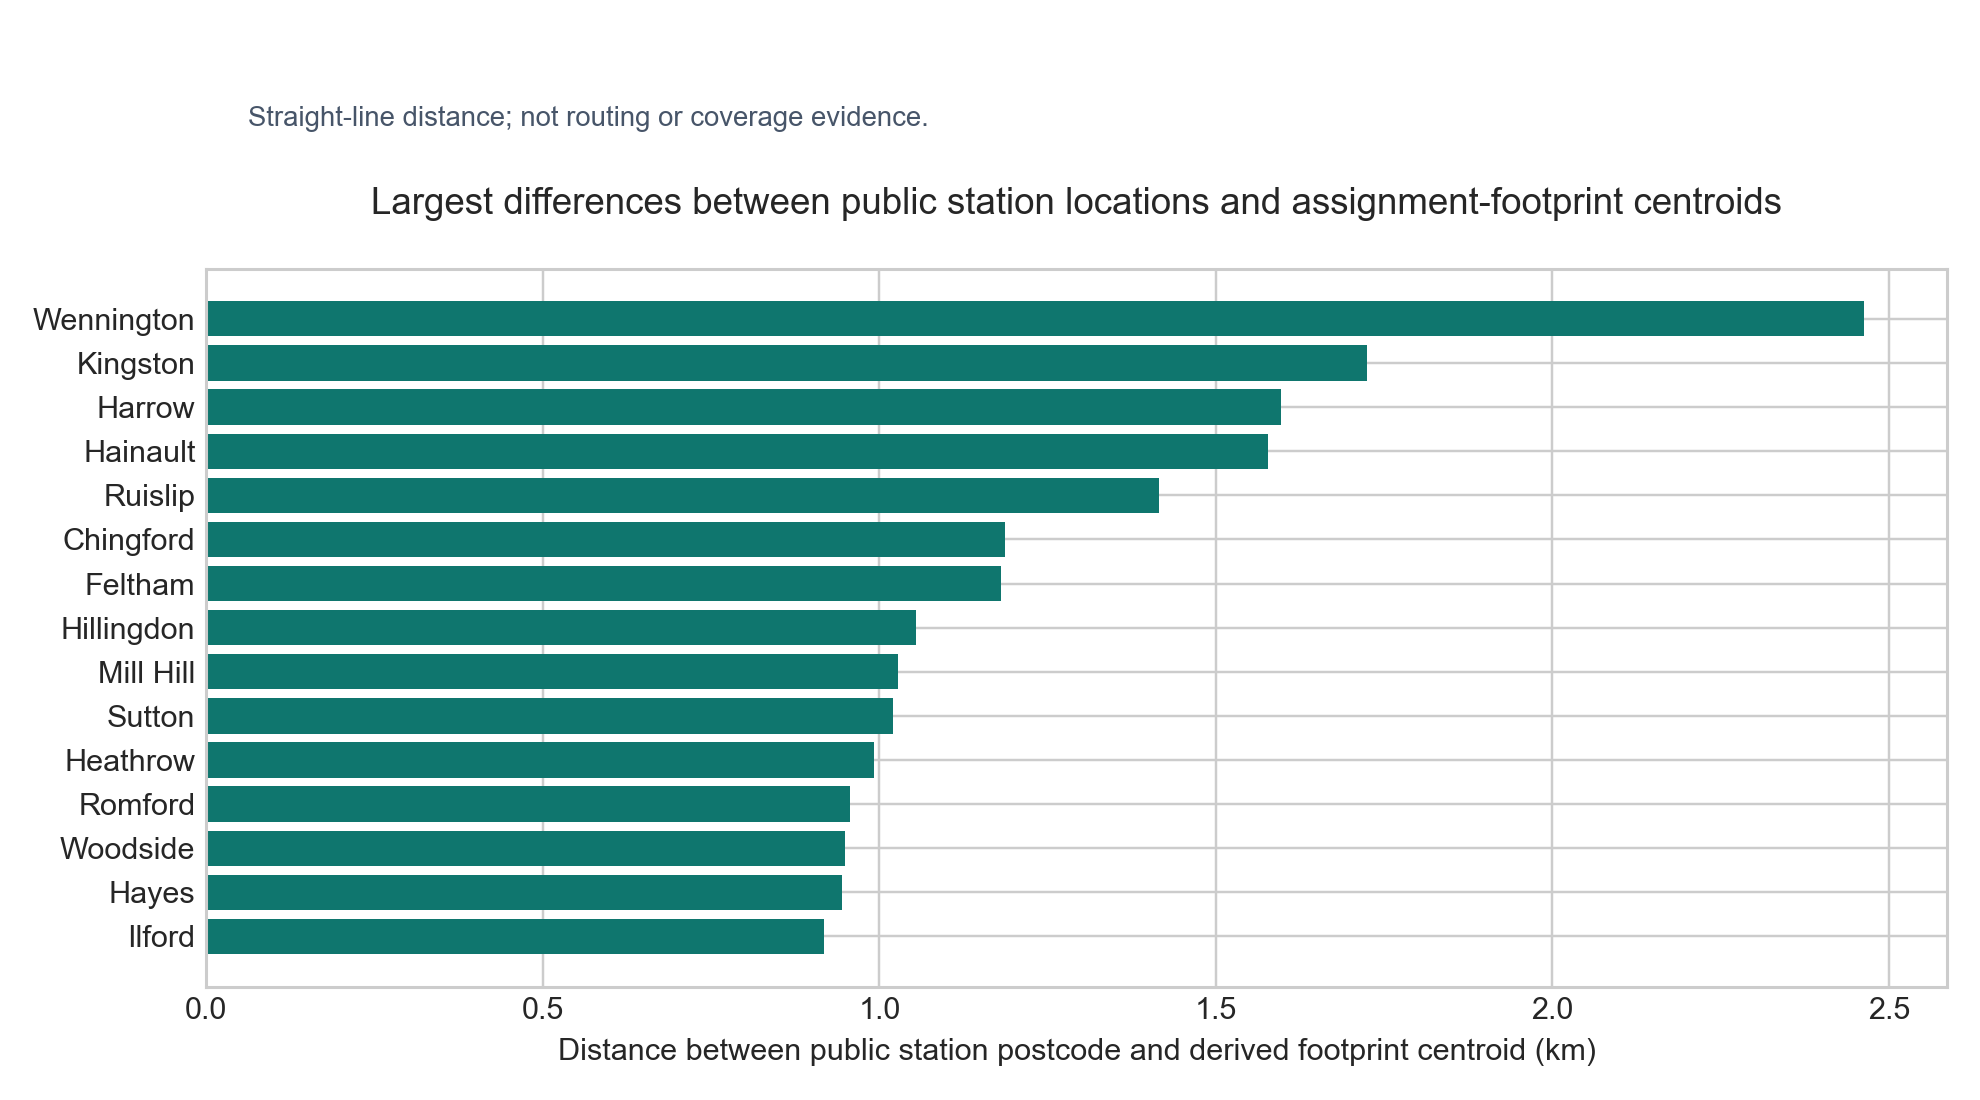
\includegraphics[width=\textwidth]{figures/station_proximity/fig_station_d1_anchor_shift_top15.png}
\caption{Largest public-address versus incident-footprint shifts among matched stations. The chart quantifies why the incident-derived footprint centroid should not be presented as a fire-station building location.}
\label{fig:station-d1-shift}
\end{figure}

The historical June 2017 source file contains 104 address rows; its page describes the LFEPA data as correct to June 2016. Of those names, 102 match assignment-footprint labels in the 2024--2026 incident slice, while Lambeth River and Merton do not. The median address-to-footprint shift is 0.43\,km and p90 is 0.99\,km. These are source-row and label-match counts, not a current operating-station total.

\begin{figure}[H]
\centering
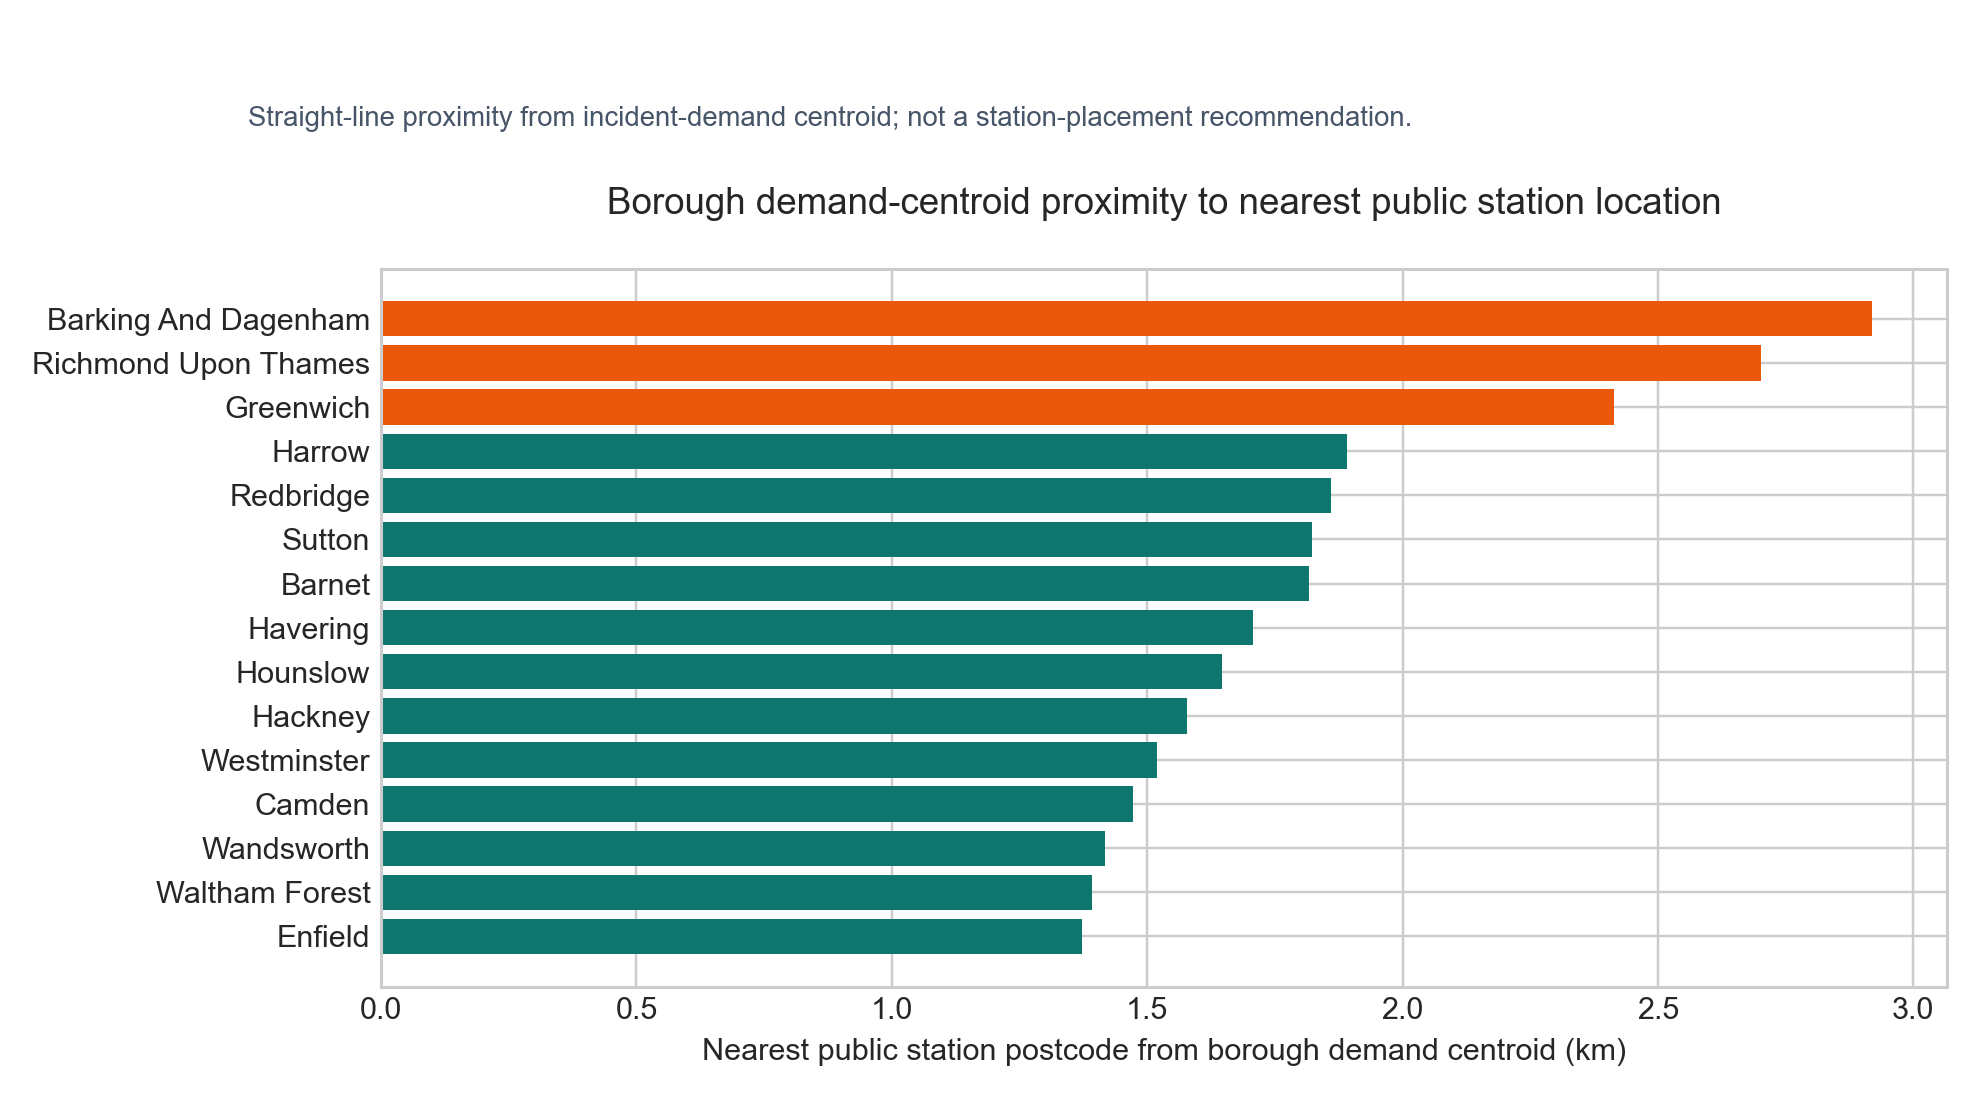
\includegraphics[width=\textwidth]{figures/station_proximity/fig_borough_nearest_station_proximity.png}
\caption{Straight-line distance from each borough incident-demand centroid to the nearest historical public fire-station postcode coordinate.}
\label{fig:borough-station-proximity}
\end{figure}

At borough level, the nearest historical station postcode coordinate to each incident-demand centroid has a median straight-line distance of 1.36\,km and a maximum of 2.92\,km. The highest-distance boroughs are Barking and Dagenham, Richmond upon Thames, Greenwich, Harrow, and Redbridge. These centroid distances describe proximity; they contain no road travel time or live availability.

\subsection{Dashboard Usability: Representation and Interaction}

The dashboard implements the core linked-view behaviours needed for RQ3: a map selection updates the trend, distribution, and ranking panels; filter controls re-render the same state; and empty selections render a visible empty state. Figure~\ref{fig:dashboard-overview} gives the whole layout, while the component captures below show the trend and ranking at report scale.

\begin{figure}[H]
\centering
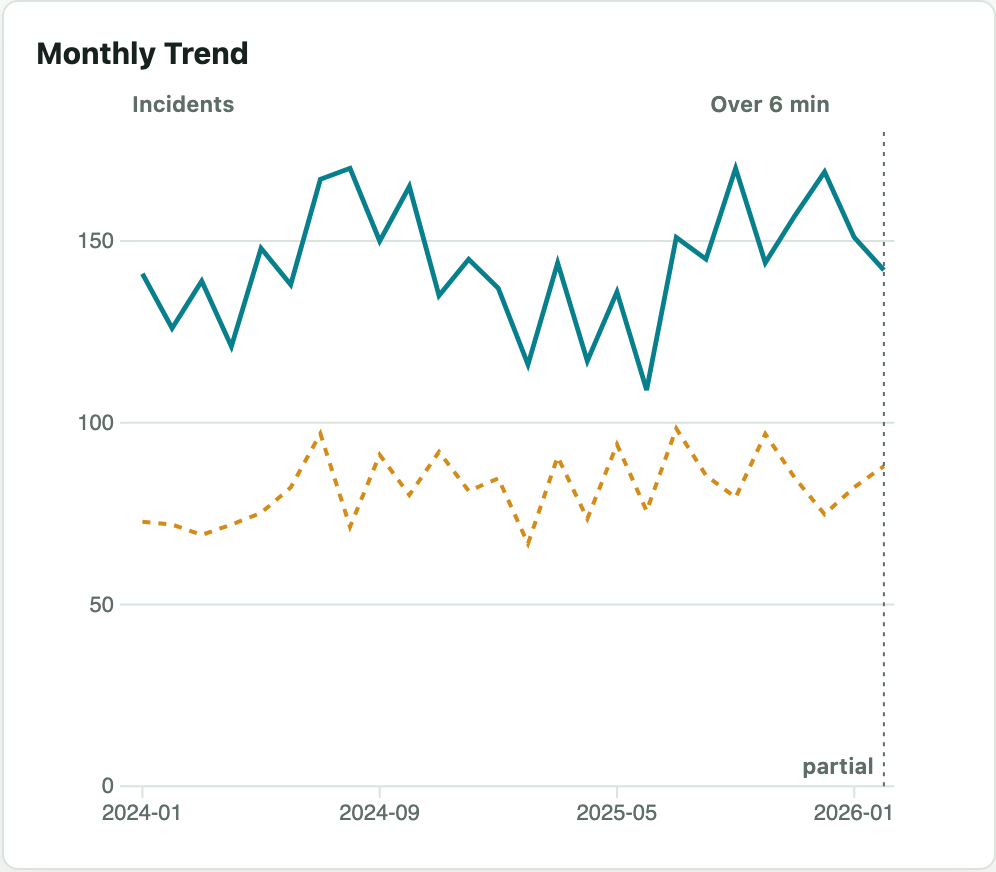
\includegraphics[width=0.82\textwidth]{figures/dashboard/fig_dashboard_trend_panel.png}
\caption{Monthly trend for a selected borough and group. February 2026 is marked partial because the source ends on 27 February.}
\label{fig:dashboard-trend-panel}
\end{figure}

The ranking table exposes exact values, recorded denominators, and 95\% Wilson intervals beside the map. Cells below 30 recorded times carry a small-sample marker. Precise-coordinate availability is not shown here because the borough aggregate uses the published borough field; that issue belongs to point-level mapping.

\begin{figure}[h]
\centering
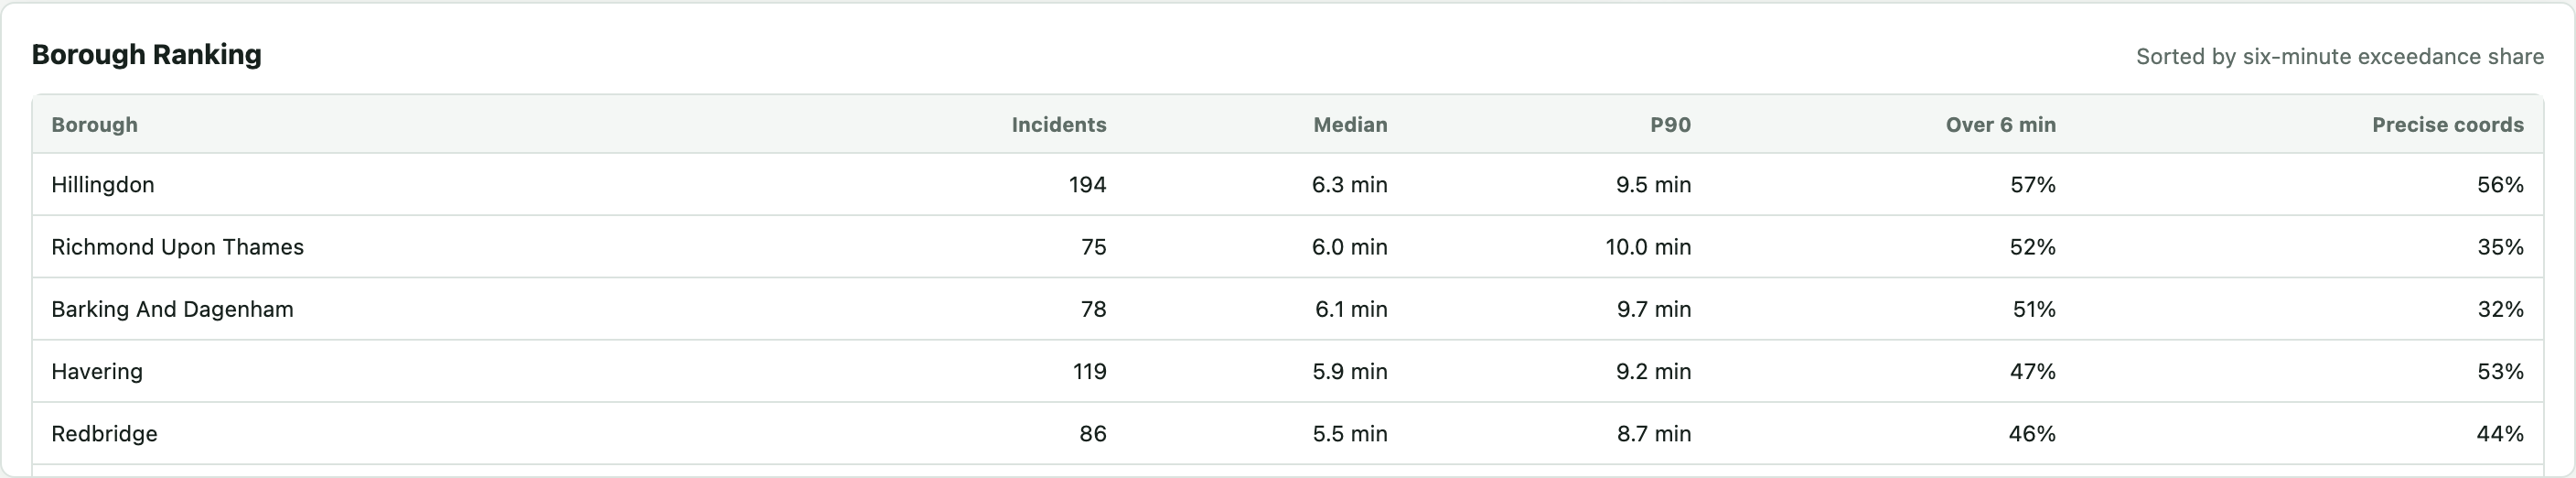
\includegraphics[width=0.86\textwidth]{figures/dashboard/fig_dashboard_ranking_table.png}
\caption{Ranking table with recorded denominators and 95\% Wilson intervals. The February 2026 state is marked partial and small recorded samples carry a warning.}
\label{fig:dashboard-ranking}
\end{figure}

The first-iteration interface still has limits. The footprint-scenario API is tested, but station-removal scenarios are not yet exposed through a front-end toggle, so the dashboard does not support browser-based station-scenario comparison. The mobile screenshot also shows that the interface is responsive enough for inspection, but this thesis treats desktop use as the primary evaluation context because the visual task involves comparative maps, trends, and tables.

\subsection{Added Value over Non-Interactive Baselines}

Table~\ref{tab:baseline-value} compares the dashboard with four non-interactive alternatives. The comparison covers implemented functions and measured latency; a controlled user comparison remains future work (\S8.3).

\begin{table}[H]
\centering
\small
\begin{tabularx}{\textwidth}{p{3.4cm}Xp{3.6cm}}
\toprule
Baseline & What the dashboard adds & Report reference \\
\midrule
Static borough choropleth & Linked ranking table and hover values show the recorded denominator and interval behind each colour. & Figures~\ref{fig:dashboard-overview}, \ref{fig:dashboard-ranking}; Table~\ref{tab:task-evaluation-matrix} path 1 \\
Raw LFB spreadsheet & The 293{,}646-row table is impractical to compare manually; pre-aggregated cells behind borough/month/incident-group filters return comparisons at interactive latency (1.1--17.7\,ms API response, \S5.3; 39.3\,ms measured click-to-update, Strand 1 record in Appendix~B). & \S5.2--\S5.3; API contract tests \\
Station-footprint map alone & The public station-address proximity layer quantifies the footprint-versus-address gap (median 0.43\,km, p90 0.99\,km), so the footprint layer cannot be silently read as station coverage. & Figures~\ref{fig:station-d1-shift}, \ref{fig:borough-station-proximity} \\
Single aggregate response median & Median--p90--p95 ranges and the author-derived proportion expose the tail that a median alone hides. & Figure~\ref{fig:incident-group-response-distribution} \\
\bottomrule
\end{tabularx}
\caption{Implemented dashboard functions compared with four non-interactive baselines.}
\label{tab:baseline-value}
\end{table}

\subsection{Data Quality and Uncertainty}

Four distinct issues affect interpretation. \emph{Variability} is the spread of observed response times and is described by median, p90, and p95. \emph{Missingness} concerns absent first-pump times and suppressed precise coordinates; it changes denominators or limits point-level maps. \emph{Proxy error} comes from rounded coordinates, postcode centroids, and incident-derived footprints. \emph{Statistical uncertainty} is finite-sample uncertainty around a recorded-time proportion; it is shown by Wilson intervals and the recorded-$n<30$ flag. None of these substitutes for another.

\begin{figure}[h]
\centering
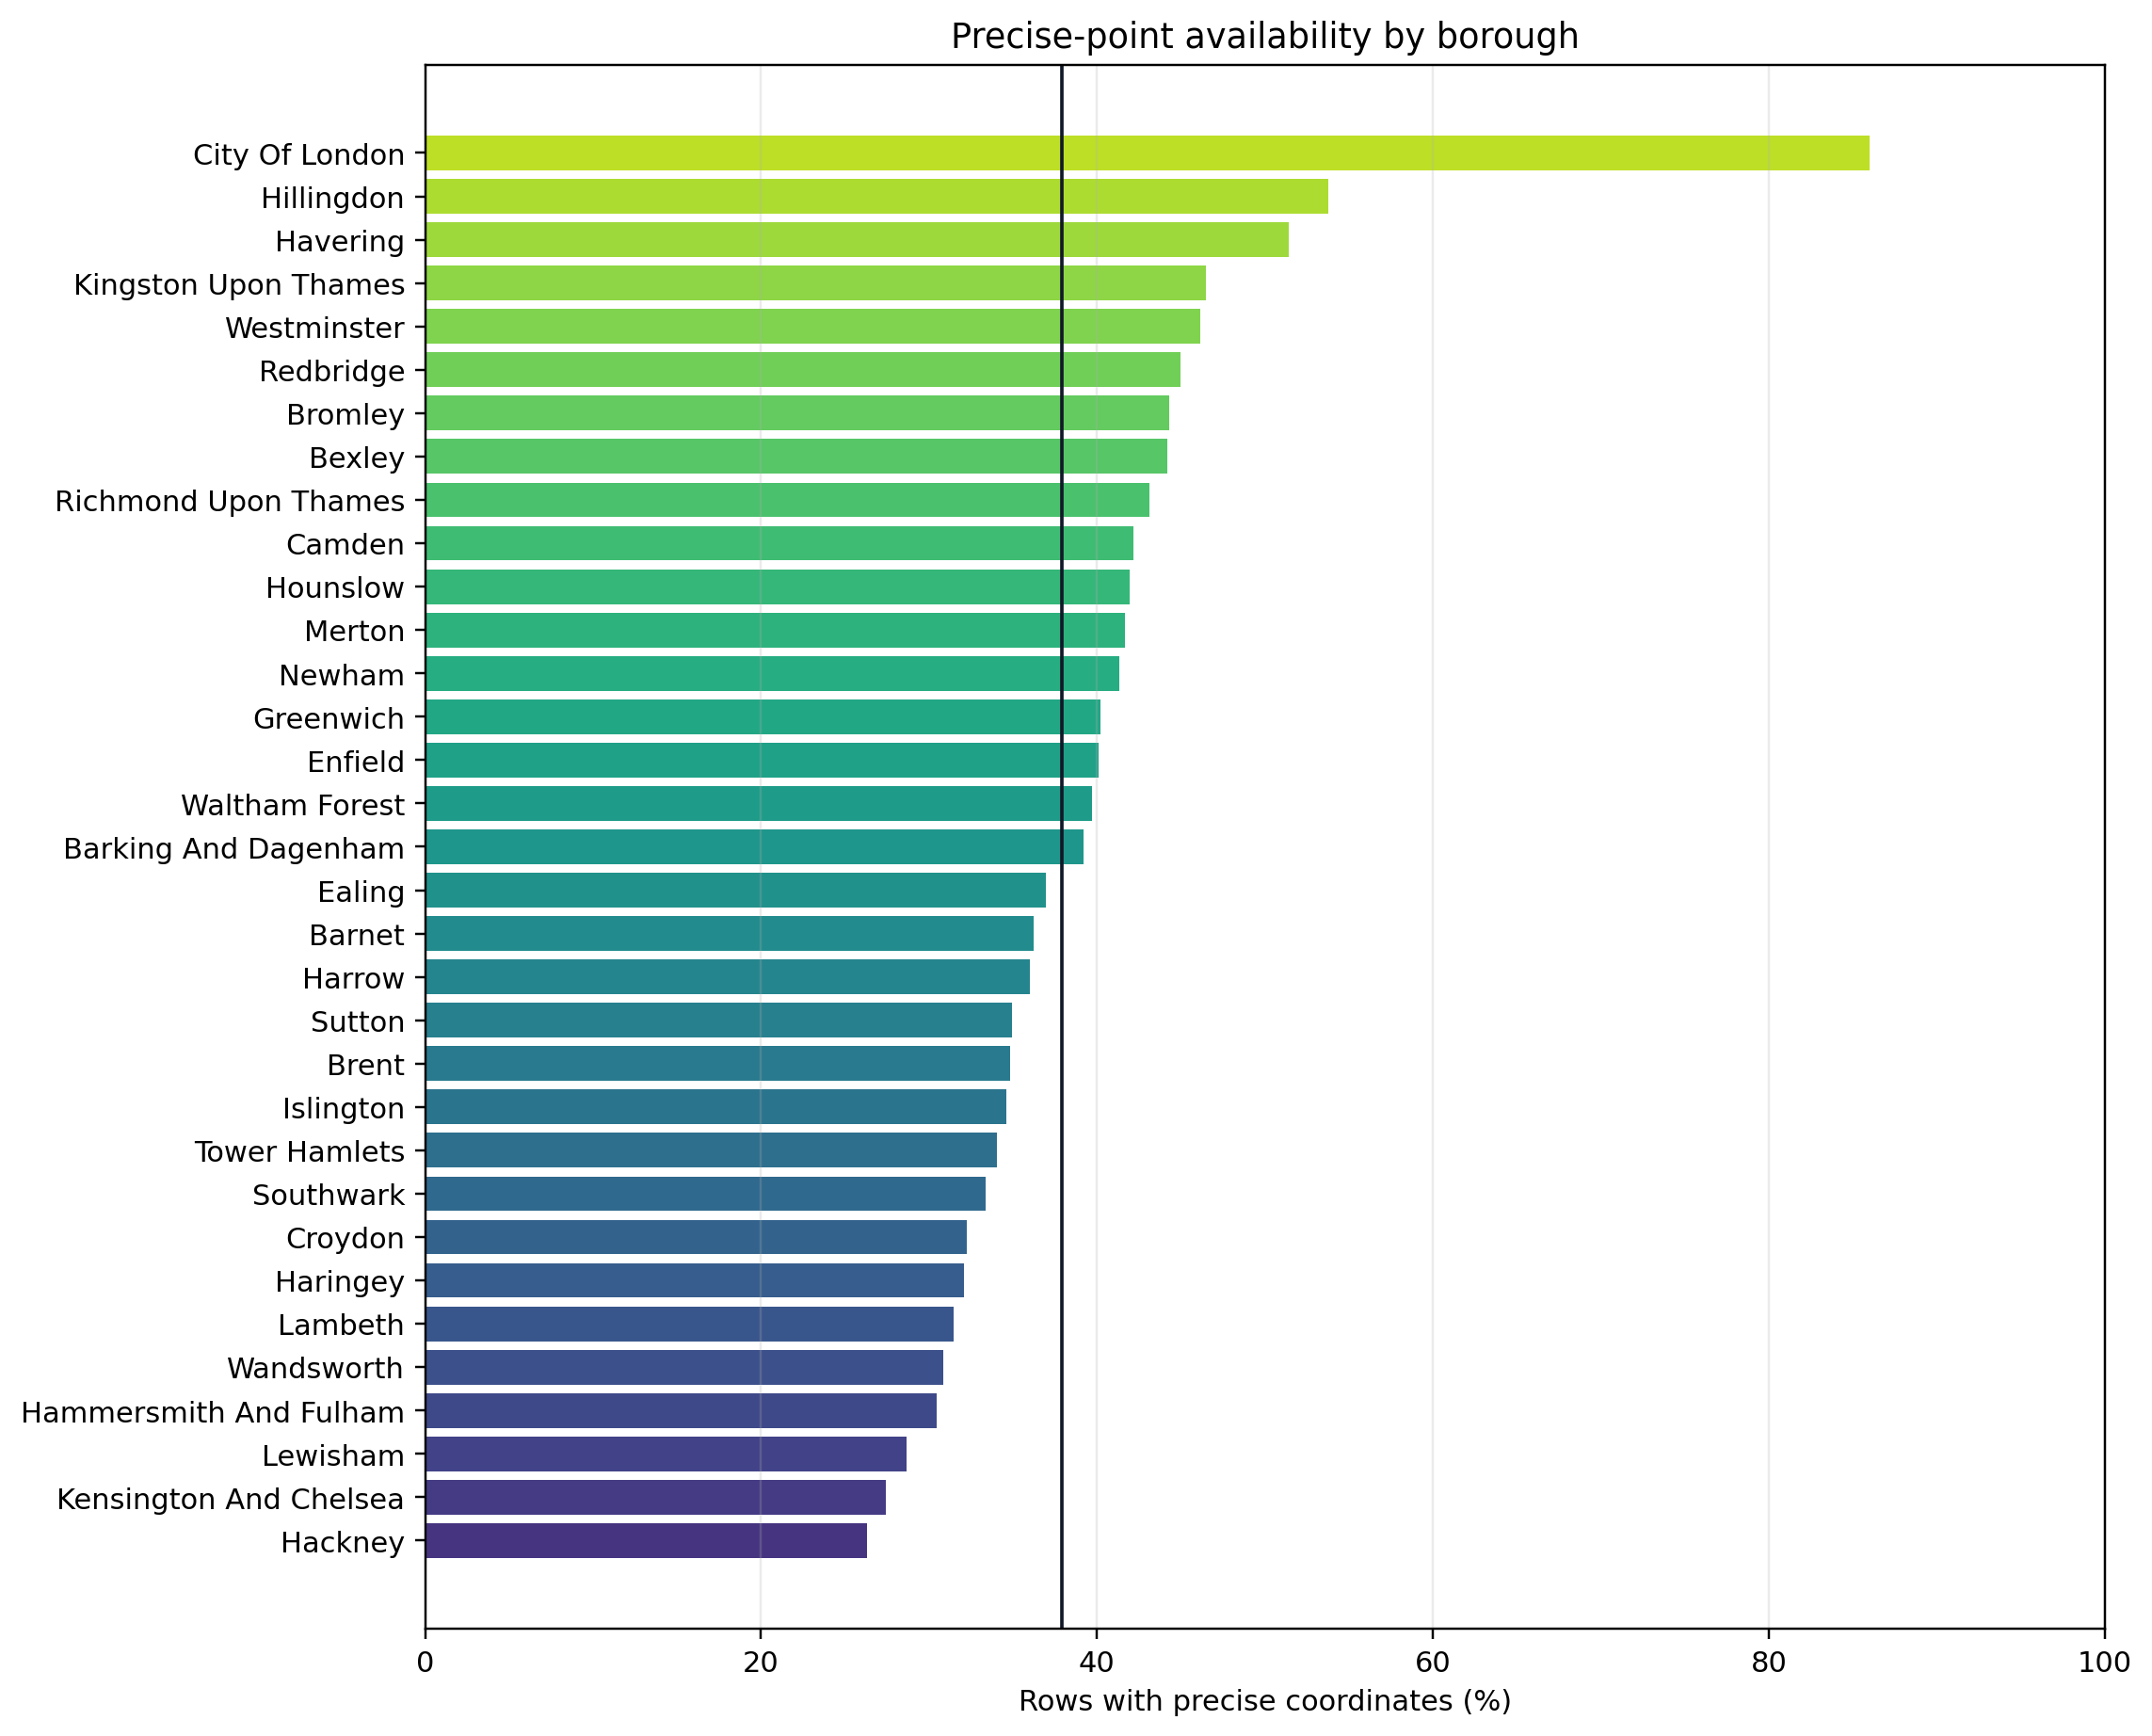
\includegraphics[width=0.92\textwidth]{figures/results_evaluation/fig_precise_coordinate_coverage_by_borough.png}
\caption{Precise-point availability by borough. This describes the subset available for point-level diagnostics; it does not condition borough aggregates.}
\label{fig:precise-coordinate-coverage}
\end{figure}

Figure~\ref{fig:precise-coordinate-coverage} shows that precise-point availability is not uniform: it ranges from 26.3\% in Hackney to 86.0\% in City of London. This limits the precise-subset density map. It does not qualify borough counts or response summaries, which use \path{borough_canonical}. Rounded points are nearly complete but still carry displacement error, so they are not described as bias-free.

\begin{figure}[h]
\centering
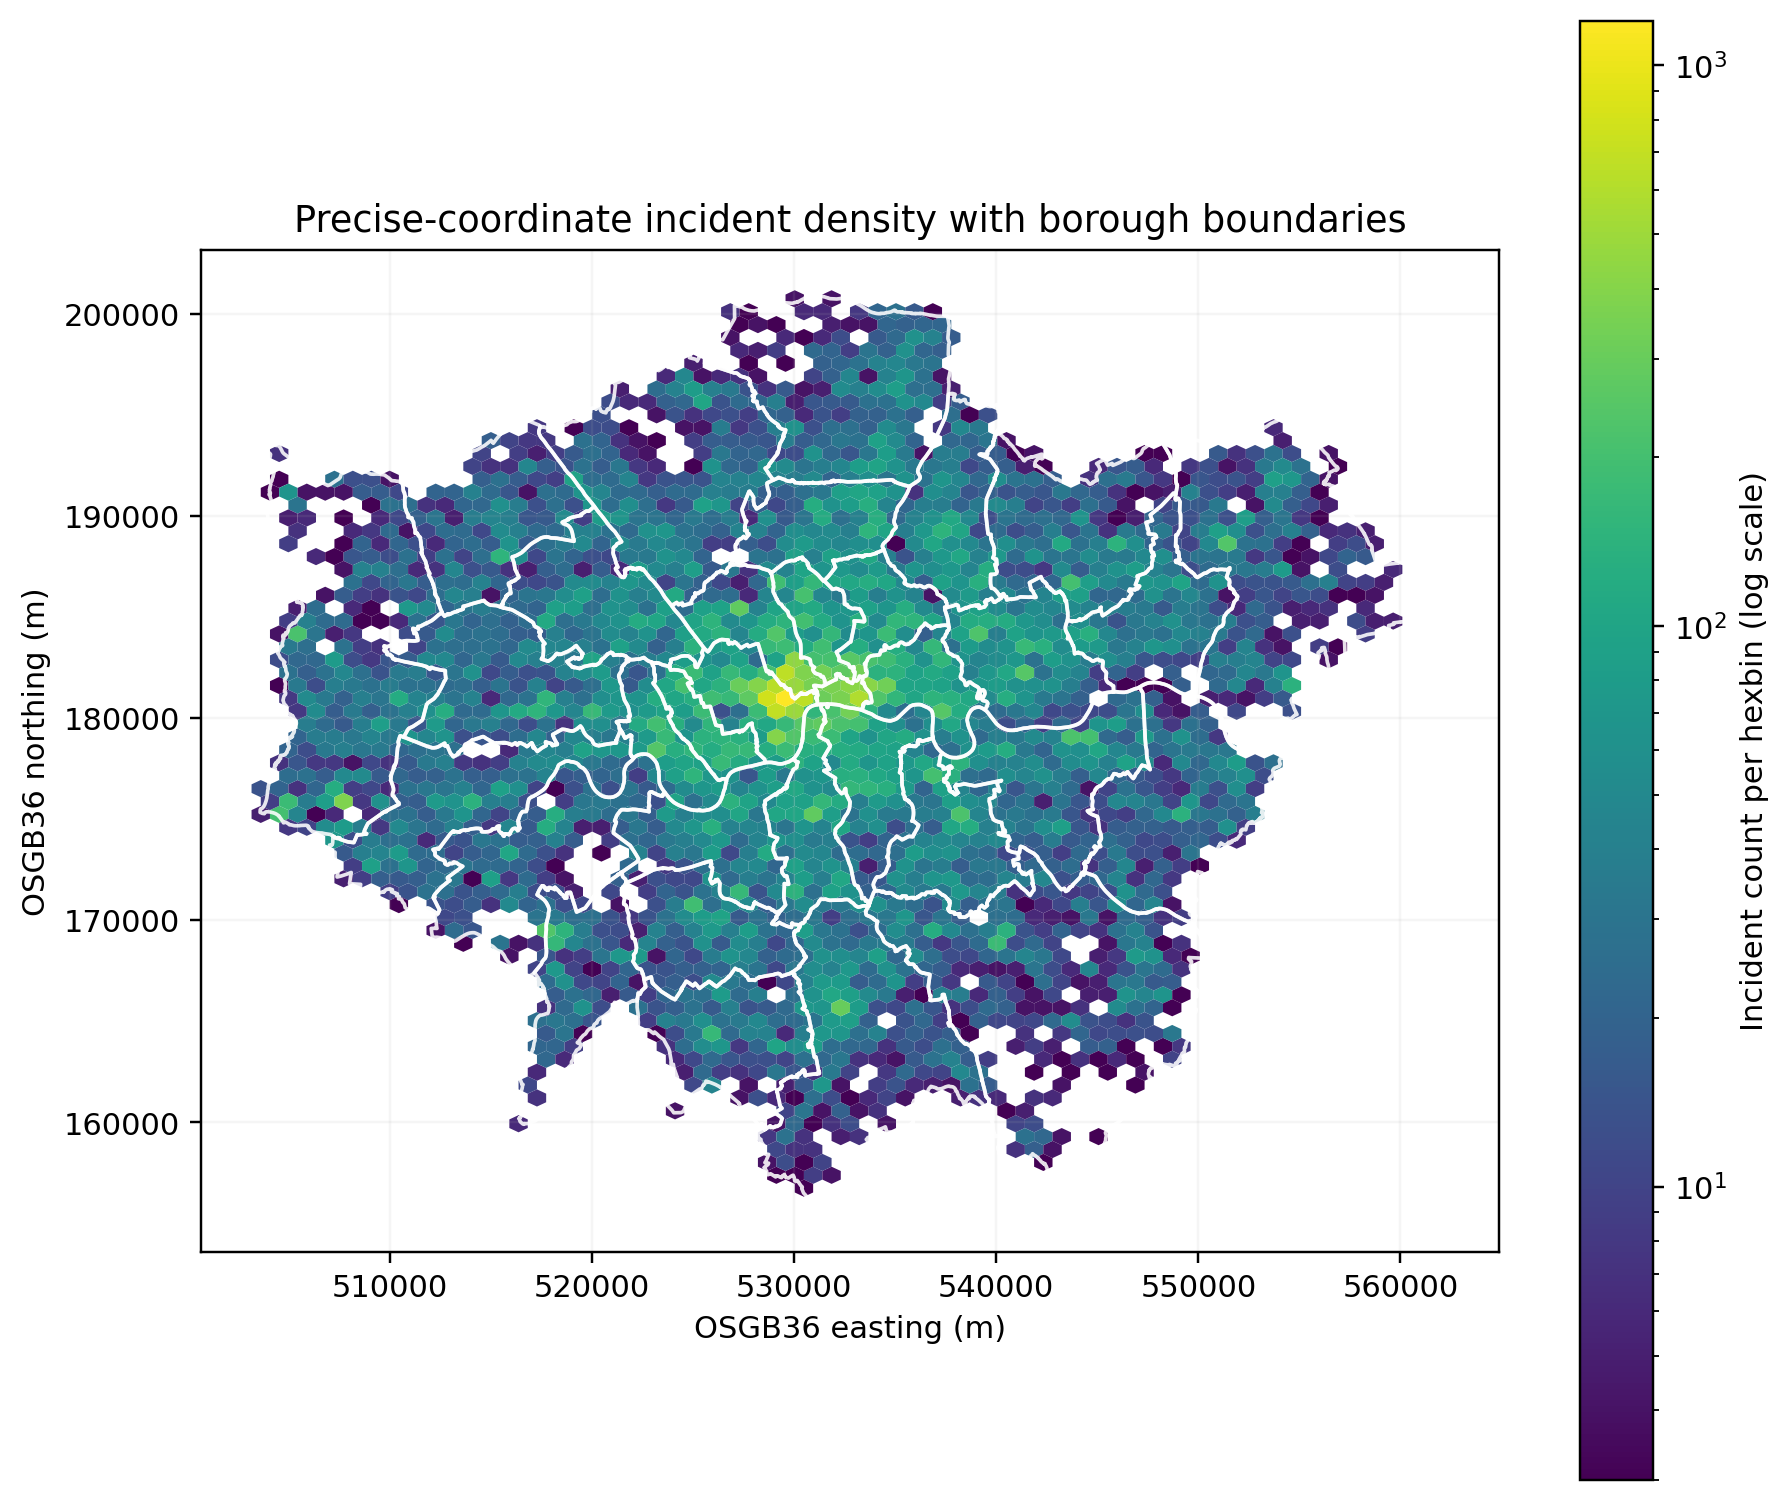
\includegraphics[width=0.82\textwidth]{figures/results_evaluation/fig_precise_spatial_density_hexbin.png}
\caption{Hexbin density for the precise-coordinate subset (37.9\% of rows). The surface reflects both incidents and point availability; it is not a full demand map. Boundaries contain National Statistics and Ordnance Survey data © Crown copyright and database right 2015~\cite{ons_boundaries}.}
\label{fig:precise-spatial-density}
\end{figure}

The precise-subset map in Figure~\ref{fig:precise-spatial-density} is a diagnostic only. Its visible density reflects both incidents and the uneven availability of precise points. Borough estimates remain separate and use the source borough label.

The dashboard now exposes the recorded denominator, Wilson interval, small-sample warning, and partial-month status. Coordinate missingness and proxy error stay beside the point-level figures, while the matched-mobilisation rule remains report/API-side. Fuzziness and quantile dotplots are future work because neither is implemented in the current interface.

\subsection{Requirement Status}

Table~\ref{tab:req-traceability} records the implemented portion and remaining work for each functional requirement.

\begin{table}[H]
\centering
\small
\begin{tabularx}{\textwidth}{p{0.7cm}p{1.2cm}p{4.2cm}X}
\toprule
Req. & Status & Delivered & Not delivered \\
\midrule
F1 & Partial & Response-diagnostic choropleth; borough/month/group filters; ranking table & Demand choropleth and year/weekday/hour filters \\
F2 & Partial & Linked monthly incident-count and exceedance-diagnostic traces & A direct monthly response-time trace as originally specified \\
F3 & Partial & Median-to-p95 ranges by incident group & Full distribution, variance view, or quantile dotplot \\
F4 & Partial & Footprint API and report-side historical address/proximity analysis & Station context in the dashboard UI \\
F5 & Partial & Recorded denominators, Wilson intervals, small-$n$ and partial-month flags; report-side coordinate/mobilisation caveats & A single UI encoding covering every missingness and proxy field \\
\bottomrule
\end{tabularx}
\caption{F1--F5 status against the requirements as originally written. ``Partial'' distinguishes implemented subsets from deferred features.}
\label{tab:req-traceability}
\end{table}

\subsection{Task-Based Evaluation}

The completed sessions used four tasks plus an uncertainty probe. A retrospective capability check found that parts of the script asked for interactions the dashboard did not provide. Those parts are treated as protocol defects, not successful system tasks.

The capability check identified four limits:
\begin{itemize}
    \item Task~1 asked for the two highest incident counts, but neither the map nor the fixed-order table ranks demand. A manual scan is possible; the ranking task is not implemented.
    \item Task~2 can compare medians through the table or tooltip. The choropleth cannot do this because it encodes an exceedance proportion, not the median.
    \item Task~3 asked users to sort the table and identify incident ``density''. Interactive sorting and a density layer are absent. The revised task uses the existing order and compares visible counts with the response diagnostic.
    \item The empty-cell question is hypothetical because all 2{,}574 cells are populated, and the station prompt uses the report-side figures rather than the dashboard screen.
\end{itemize}

\begin{table}[H]
\centering
\small
\begin{tabularx}{\textwidth}{p{2.4cm}p{3.2cm}p{4.3cm}X}
\toprule
User path & Task focus & Observed issue & Recorded result \\
\midrule
Map-first analyst & Compare Hillingdon with an inner-London borough using map, trend, and ranking table & Uses the table to move from colour impression to an exact recorded-denominator comparison. & Supported by the implemented linked views. \\
Table-first policy reader & Interpret response-performance ranking & Uses exact values, but initially reads the proportion as applying to all incidents. & Supports the clearer recorded-$n$ and interval wording. \\
Station-context reader & Interpret the two station references & Initially confuses the assignment footprint with the public address, then separates them after reading the scope note. & Correctly distinguishes the two sources after the prompt. \\
\bottomrule
\end{tabularx}
\caption{Task-based evaluation matrix used to connect dashboard actions with observable interpretation behaviour.}
\label{tab:task-evaluation-matrix}
\end{table}

The participant summary below covers how the panels were compared. Results from unsupported task mechanics are omitted from the completion assessment.

\subsection{Think-Aloud Summary}

The compact think-aloud evaluation involved three voluntary participants, anonymised here as Participant~1--Participant~3. Each participant completed a task-based inspection of the dashboard while verbalising their interpretation of the linked map, trend, distribution, and ranking views. The observation notes focused on comparison behaviour, uncertainty noticing, denominator checking, and interpretation of station context. No sensitive personal data were collected, and the results are treated as a small-scale formative interpretability check rather than as a statistically generalisable user study.

Table~\ref{tab:thinkaloud-summary} reproduces the participant-level aggregate stored in the evaluation summary. Per-session notes are not included in the submitted workspace, so the table cannot be independently reconciled to raw logs here.

\begin{table}[H]
\centering
\small
\begin{tabularx}{\textwidth}{p{2.3cm}XX}
\toprule
Participant & Observed behaviour & Interpretation for RQ3 \\
\midrule
Participant 1 & \textbf{Linked-view validation:} map-first path; all tasks completed; Hillingdon selected; tooltip used for recorded-time denominator. & \textbf{Qualified comparison:} colour cue converted into table/tooltip-supported claim; station-coverage overclaim avoided. \\
Participant 2 & \textbf{Label-friction case:} table-first path; Tasks 1--3 completed; one prompt needed for month comparison; ``precise coords'' label queried. & \textbf{Uncertainty wording gap:} exact values useful, but denominator and station-proximity caveats require stronger first-encounter wording. \\
Participant 3 & \textbf{Cautious-trend path:} trend-first path; all tasks completed; risk judgement stated as tentative; missing response times volunteered. & \textbf{Structured comparison:} dashboard supports comparison, but coordinate coverage remains probe-dependent; dashboard alone not read as station coverage. \\
\bottomrule
\end{tabularx}
\caption{Small think-aloud aggregate used to interpret the dashboard's support for qualified comparison.}
\label{tab:thinkaloud-summary}
\end{table}

The aggregate suggests that different starting panels still led to borough comparisons. Denominator awareness was mixed, supporting the clearer recorded-$n$ wording. The coordinate-coverage prompt also exposed a design error: it encouraged users to connect point availability with a borough estimate that does not use points. That column has therefore been replaced by the confidence interval. Station context remained understandable only with the report-side figures. These interface changes were made after the sessions; they are covered by system tests and the updated walk-through, but have not been participant-tested.

\subsection{Evaluation Limitations}

The evaluation is formative and small. The submitted workspace contains the instruments and aggregate summary but no per-session notes, so participant-level details cannot be re-audited from the repository alone. Task~1 and Task~3 also asked for mechanics the interface did not provide. The completed paths show usable linked borough comparisons, while denominator and station-context wording sometimes needed prompts.
